In this chapter, the process of designing the front-end sampling card is described.
Designing a \gls{pcb} is a two step process: circuit design and layout design.
In this thesis, the software used to cover both of these steps is PADS xDx Designer (for schematic capture) and PADS Layout/Router (for \gls{pcb} layout design) from Mentor Graphics (subsidiary of Siemens).

\section{Schematics}
Without knowing which components are needed and how they are interconnected, it is impossible to manufacture any board, no matter how high or low the level of complexity is.
The main purpose of a schematic is thus to provide a documentation about the necessary components and in which way they should be connected to another.
Furthermore, a schematic provides a starting point for automatic placement and routing, i.e. where the components are placed and how they are connected on the physical \gls{pcb}, which is done with the layout design tool.
During the creation of the schematics, the following points have to be taken into consideration:

\begin{itemize}
	\item Deciding which components are needed and what the performance requirements are. Especially for high-speed components carefully considering specifications like signal rise and fall times, jitter, skew, etc. is crucial to achieve the overall expected performance.
	\item Keeping in mind how many pins are available for peripheral connection, control signals, etc. Many components have an interface for programming (e.g. \gls{spi}) which requires several pins. Especially for boards with a lot of components this can quickly become an issue.
	\item Checking the signaling interfaces of the components. Additional circuitry might be needed for interfacing between two different components. Some signaling interfaces, like \gls{lvds}, require a specific voltage level, which might result in the need of voltage level translators.
	\item Keep in mind the different common mode voltages at input/output pins of different components and placing decoupling capacitors if needed.
	\item Consider placing additional filtering for power supplies, as well as recommended filters from manufacturers of the components. 
	\item Choose suitable type and amount of power supplies/voltage regulators.
	\item Packaging/Size of the components. Obviously the size matters, as space on the board is limited. But the package also introduces additional capacitance/inductance, which can be a problem for precise filtering circuits. 
	\item Power dissipation of the components. Especially voltage regulators might need coolers. This might not pose any problems for components which are located on the top side of the board. However, components on the bottom side might create an issue, if the designed \gls{pcb} should be mounted on another board.
	\item For mixed-signal boards, i.e. boards containing digital and analog signal paths, analog and digital ground should be separated. For \glspl{ic} like \glspl{tha} or \glspl{adc}, where both analog and digital signals are present, connecting the grounds via appropriate components needs to be considered.
	\item Check if the components are still available and if they can be delivered in the given project time.
\end{itemize}  

This list is certainly not complete, but provides an overview over the most important points which need to be taken into account during design.
Decoupling techniques and separation of analog and digital ground are explained a bit more detailed, being very important and crucial steps for design of high-performance \gls{pcb}.
%todo irgendeine überleitung hinschreiben
 
\paragraph{Decoupling techniques}
Probably the most important part in schematics design is proper decoupling of power supplies, as \glspl{ic} require a stable voltage on the power supply pin for optimal performance.
Any ripple\footnote{\textit{Ripple} is the \gls{ac}-voltage superimposed on an otherwise \gls{dc}-voltage.} or noise can substantially degrade the performance of the \glspl{ic}, i.e. by decreasing the noise margin.
\textit{Noise margin} defines the difference between the useful signal and noise. 
A sufficient noise margin is necessary to guarantee that the output signal will still be correctly interpreted, even if some noise is added to the signal.
Usually, manufacturers give information about proper decoupling circuits for their component in the data sheet.
If this is not the case, there are basic rules of thumb which can be followed to ensure good decoupling. \cite{decouple}

Basically, two types of voltage variations on the power supply pin can be distinguished: low frequency and high frequency variation.
Low frequency variation occurs for example due to devices (or parts of them) being enabled/disabled or in the event of data traffic or data processing.
The current draw during these occurrences can not be compensated immediately by the voltage regulator providing the supply voltage, which leads to drops in the voltage levels.
Time frames of this variation vary in the range of milliseconds up to days.
High frequency variation results from switching events in the device, occurring in the range of the clock frequency and the corresponding harmonics up to about \SI{5}{\giga \hertz}.
Spikes due to \gls{emi} are also a source of high frequency variation and need to be compensated for. \cite{xilDecouple} 

Ideally, one capacitor, which acts as a low-pass filter, should be enough to mitigate these variations.
A real capacitor however has parasitics and thus can in general not be modeled by a ``pure'' capacitive behavior, especially for high-frequency applications. %todo define parasitics
Additional resistances and inductance need to be considered \cite{decouple}:
\begin{itemize}
	\item A parallel resistance $R_P$, which shunts the nominal capacitance ($C$), representing insulation resistance or leakage.
	\item A series resistance $R_S$, or \gls{esr}, which represents the plates and the leads of the capcitor.
	\item A series inductance $L_S$, or \gls{esl}, that models the inductance of the plates and leads of the capacitor.
	\item A parallel resistance and capacitance, $R_D$ and $R_C$, which model the effect called dielectric absorption. This denotes the phenomenon, that a capacitor which has been charged for a long time, doesn't fully discharge when briefly discharged. Dielectric absorption can be detrimental for high-precision use-cases, for power supply decoupling this effect doesn't have to be considered.
\end{itemize}
Consideration of all these effects leads to the equivalent circuit shown in \autoref{fig:real_cap}.
It can be seen that this forms a RLC circuit, meaning the capacitor will not have the ideal behavior over the whole frequency range. 
In fact, a real capacitor shows an impedance response as seen in \autoref{fig:esl_esr}, which resembles one of a band stop, rather than a low pass.
Typical capacitive behavior is seen in region (I).
Region (II) shows the influence of the \gls{esr}, which is why there is a residual impedance at the lowest point.
Region (III) showcases the effect of the \gls{esl}. 
To extend the capacitive behavior over a wider frequency range, at least two capacitors are placed.

\tikzexternaldisable
\begin{figure}[tbh]
	\centering
	\includegraphics[width = .7\textwidth]{chap/04-work/img/real_cap.tikz}
	\caption[Capacitor equivalent circuit]{Equivalent circuit of a real capacitance (redrawn from \cite{decouple})}
	\label{fig:real_cap}
\end{figure}
\tikzexternalenable
\begin{figure}[tbh]
	\centering
	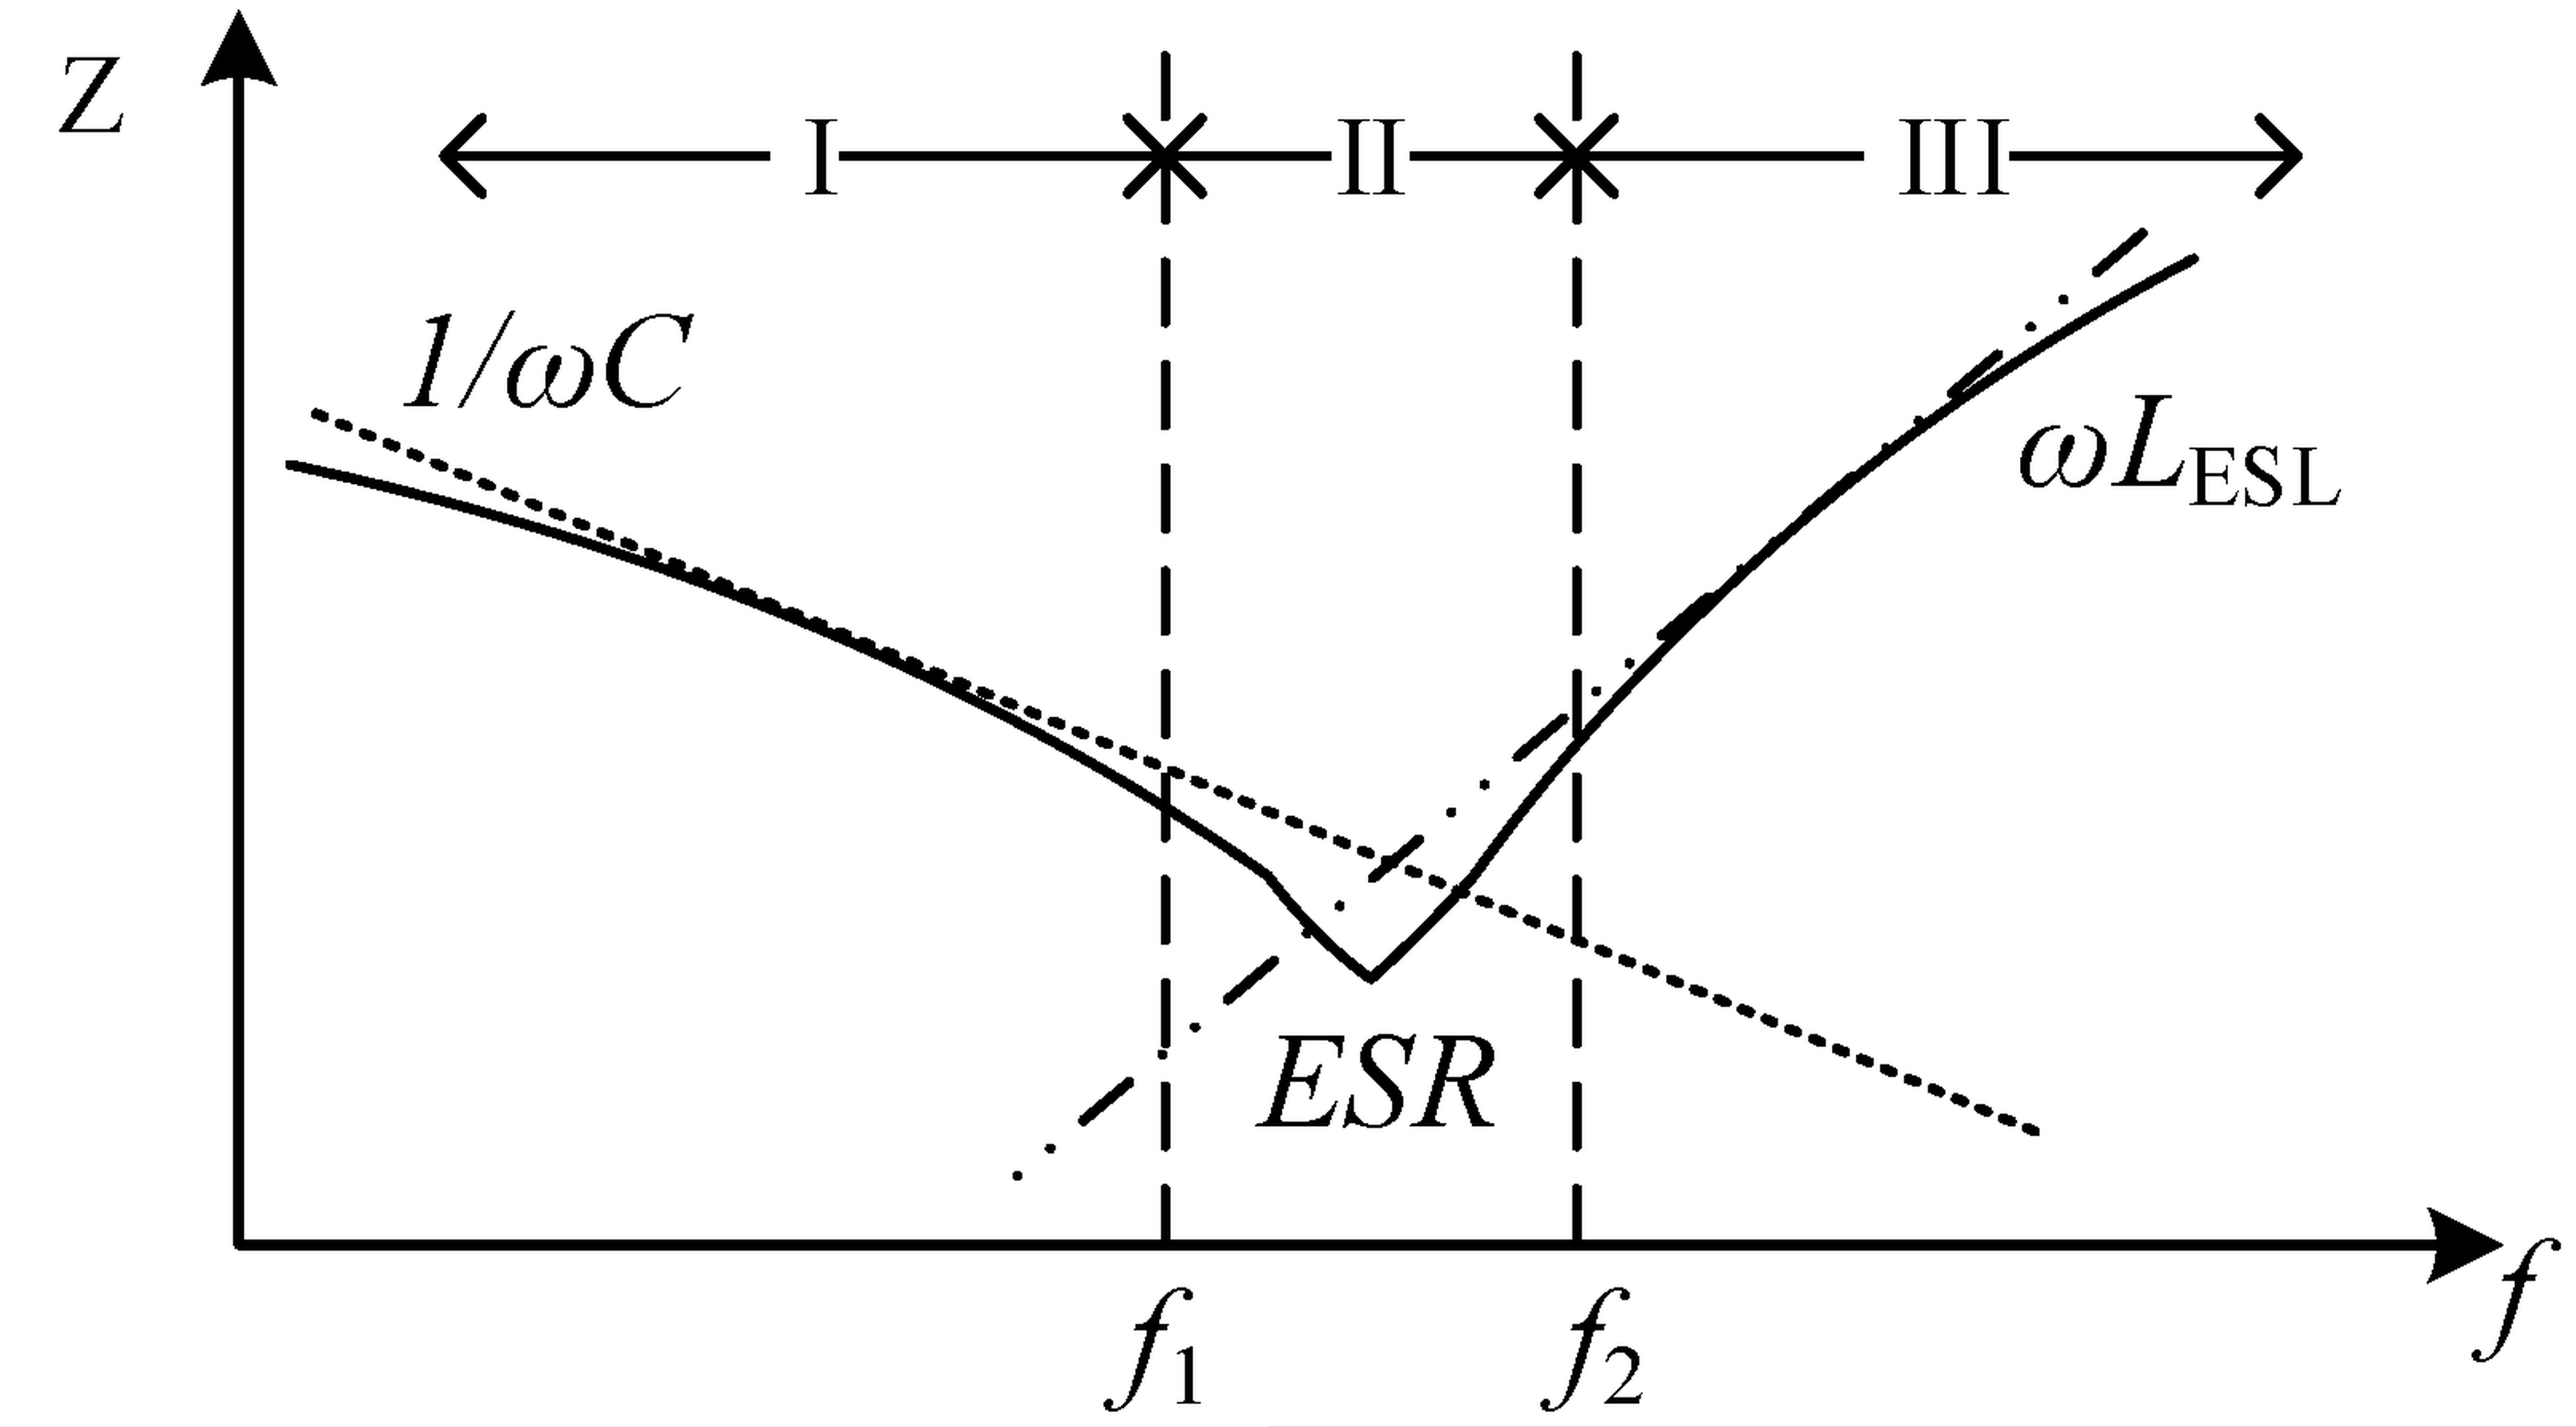
\includegraphics[width = 0.8\textwidth]{chap/04-work/img/esl_esr}
	\caption[Impedance response of a real capacitor]{Qualitative impedance response of a real capacitance \cite{Dang2020}}
	\label{fig:esl_esr}
\end{figure}


To deal with the low frequency variation, a large capacitor (typical values: \SIrange{10}{100}{\micro\farad}) is placed next to the component, not more than \SI{5}{\centi \metre} ($\approx$ 2 inch.) away.
The role of this capacitor is to be a charge supply for the instantaneous needs of the device, i.e. keeping a constant voltage level until the slower control loop of the voltage regulator can compensate for the changed current draw. \cite{decouple}

A small capacitor (typical values: \SIrange{0.01}{0.1}{\micro \farad}), placed as close as possible to the power pins of the component.
This capacitor should bypass the high frequency variation on the power supply line. \cite{decouple}

To cover a larger frequency range, multiple capacitors can be used.

All capacitors should be connected through vias or short traces to a large area, low impedance ground plane. Vias on a \gls{pcb} are used to connect different layers, a plane is an uninterrupted area of metal covering the whole (or part) of a \gls{pcb} layer (basic \gls{pcb} structures are also  explained in \autoref{ssec:pcb_structs}). 
Connecting capacitors in this way minimizes the inductance due to connection traces. \cite{decouple}

An optional ferrite bead in series with the supply pin keeps external high frequency from the device and the noise generated inside the component from the rest of the board. \cite{decouple}

\paragraph{Separating Analog and Digital Ground}
TODO

\subsection{Connectors}\label{sec:connectors}
The number and type of connectors is primarily defined by the read-out card, on which the sampling board is mounted.
The different connector types serve different purposes, which can be organized into three categories.

\paragraph{Digital Control Signals}
For digital control signals (i.e. \gls{spi}, enable signals, \ldots) and clocking a VITA 57.4 FMC+ connector from \textit{SAMTEC} is used (see \autoref{fig:fmcp}). 

\gls{fmc} is a standard defined by \gls{vita} to provide a standard mezzanine card\footnote{A \gls{pcb} which is plugged on a plug-in board. \cite{mezzanine}} form factor, connectors, and modular interface to a \gls{fpga} located on a base board (carrier card). \cite{Seelam2009}
The \gls{fmc}+ standard extends the pin count and throughput of the present high-speed interfaces. 

This connector provides 560 pins arranged in a $14\times40$ array, 80 of which are additional high-speed interfaces, located on either side of the connector (therefore this connector type is also called \gls{hspce} connector, as opposed to the HSPC connector which doesn't have additional rows).
For user-defined purpose 160 pins are available. 
They can be used as single-ended or differential pins.
Clocking capable pins can be used to propagate clock signals from the mezzanine to the carrier board. 

Furthermore, the connector provides pins for power supply from carrier board to mezzanine card. \cite{fmc} The voltage levels provided are listed in \autoref{tab:fmc_ps}.



\begin{table}[tbh]
	\caption[FMC+ Voltages]{Voltage levels for power supply provided by the \gls{fmc}+}
	\label{tab:fmc_ps}
		\centering
		\begin{tabularx}{\textwidth}{Xcc}
			\toprule
			\textbf{Voltage} & \textbf{Max. current} & \textbf{Max. capacitive load}\\
			\midrule
			$V_\text{ADJ}$, \SIrange{0}{3.3}{\volt} & \SI{4}{\ampere} & \SI{1000}{\micro \farad}\\
			\SI{3.3}{\volt} & \SI{3}{\ampere} & \SI{1000}{\micro \farad}\\
			\SI{12}{\volt} & \SI{1}{\ampere} & \SI{1000}{\micro \farad}\\
			\bottomrule
		\end{tabularx}
\end{table}

An assembly drawing of the \gls{fmc}+ connector is shown in \autoref{fig:fmcp}.

\begin{figure}[tbh]
	\centering
	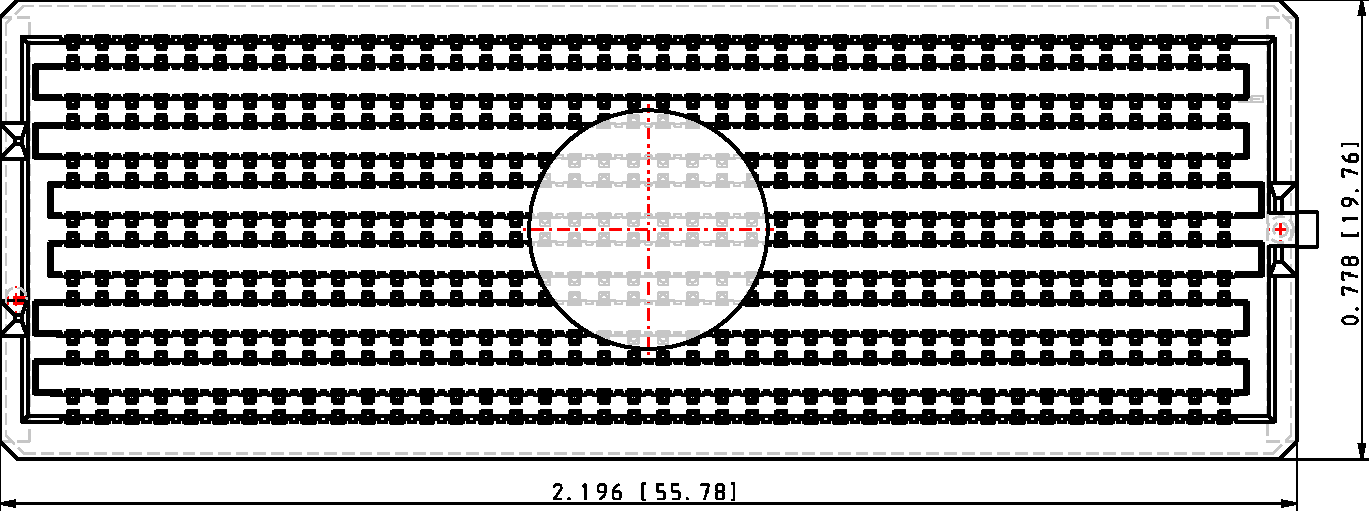
\includegraphics[width = 0.7\textwidth]{chap/04-work/img/fmcp.pdf}
	\caption[Rendering of FMC+ connector]{Part drawing of FMC+ connector \cite{fmcpic}}
	\label{fig:fmcp}
\end{figure}

\paragraph{Analog Signals}
The signal from the detector is provided to the \glspl{tha} through \gls{sma}\footnote{Coaxial \gls{rf} connector} \gls{rf} connectors from \textit{molex}, which are mounted at the edge of the board.
\autoref{fig:sma} shows a 3D model of this connector type. 

\begin{figure}[tbh]
	\centering
	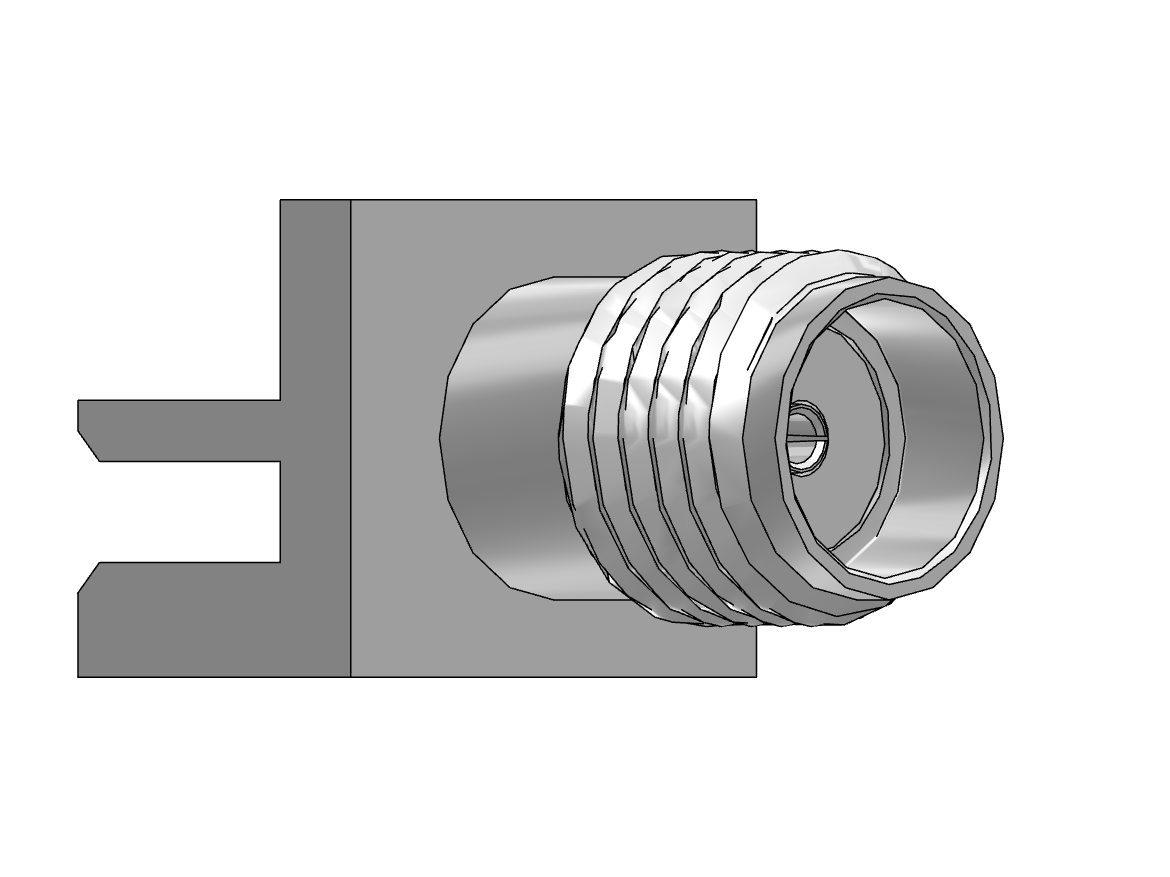
\includegraphics[width = 0.5\textwidth]{chap/04-work/img/sma}
	\caption[Edge-Mount RF SMA connector]{3D model of the edge-mount \gls{rf} \gls{sma} connector from \textit{molex} \cite{molex}}
	\label{fig:sma}
\end{figure}

On the read-out board two RFMC 2.0 (\gls{rf} Mezzanine Card) interface connectors are provided.
The connectors used are \gls{lpaf} connectors from \textit{SAMTEC} with 400 pins arranged in a $8\times50$ array.
One connector is dedicated for transmitting signals from the mezzanine card to the on-board \glspl{adc}.
The other provides the analog output from the on-board \glspl{dac}\footnote{A \gls{dac} translates digital values into an analog signal.} to the mezzanine card.
On the sampling board, the male counterpart of the connectors, \gls{lpam}, is used (see \autoref{fig:lpam1}).

\begin{figure}[tbh]
	\centering
	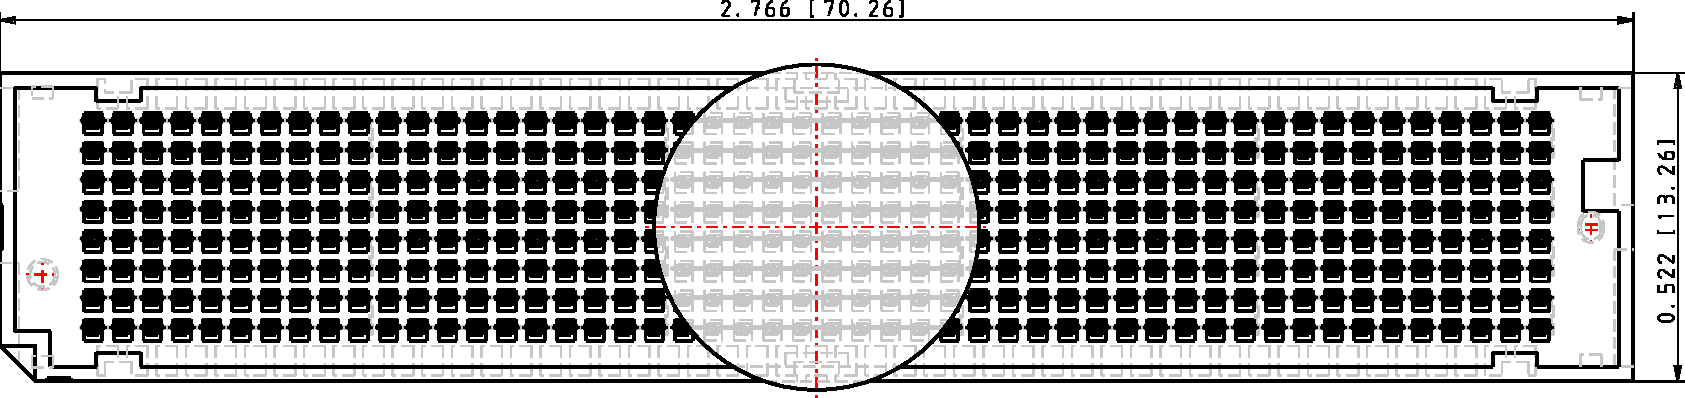
\includegraphics[width = \textwidth]{chap/04-work/img/lpam_50_top.pdf}
	\caption[LPAM $8\times50$ connector]{Part drawing of a LPAM $8\times50$ connector}
	\label{fig:lpam1}
\end{figure}


\paragraph{Clock Signals}
The clock signals from the \glspl{pll} on the sampling board are propagated in different ways.
The reference clock for the \gls{fpga} is propagated through the \gls{fmc}+ connector.
Clocking for the \glspl{adc} and the \glspl{dac} is provided through a $6\times20$ \gls{lpam} connector (see \autoref{fig:lpam2}).
\begin{figure}[tbh]
	\centering
	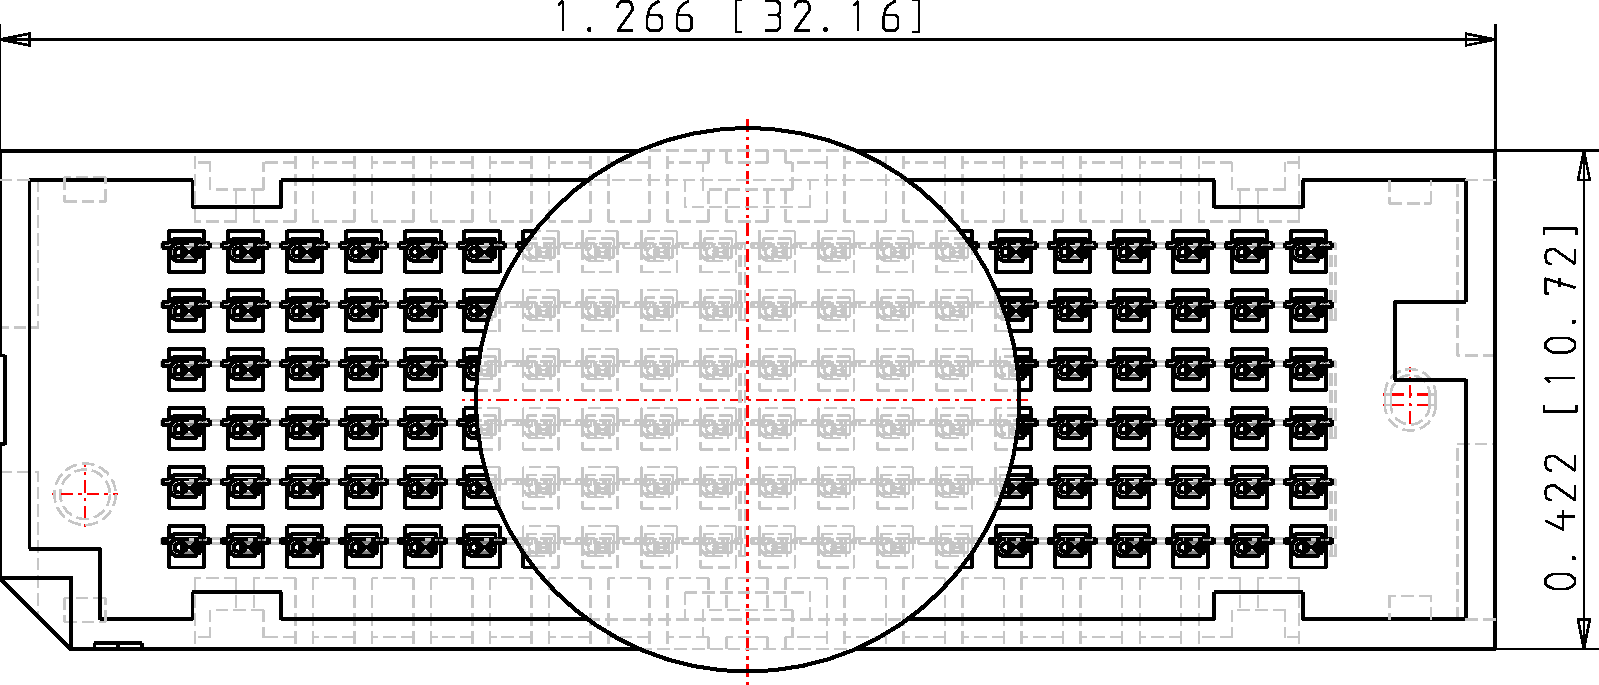
\includegraphics[width = 0.7\textwidth]{chap/04-work/img/lpam_20.pdf}
	\caption[LPAM $6\times20$ connector]{Part drawing of LPAM $6\times20$ connector}
	\label{fig:lpam2}
\end{figure}

The clock coming from \gls{kara} is provided through \gls{rf} SMA connectors directly to the \gls{pll}.

\subsection{Sampling-Channel}
The sampling channel consists of the \gls{tha}, which is driven by a delay chip. 

\paragraph{Track-And-Hold-Amplifier}
The \gls{tha} used is the same as in \gls{kapture}. The component was chosen such that jitter lies in the range of hundreds of femtoseconds. \cite{caselle2013}
According to the data sheet \cite{hmc5640}, the component shows the characteristics shown in \autoref{tab:hmc5640}.
\begin{table}[tbh]
	\caption[HMC5640 Characteristics]{Specifications of the HMC5640 \gls{tha}}
	\label{tab:hmc5640}
	\begin{minipage}{\textwidth}
		\centering
		\begin{tabularx}{\textwidth}{Xcccc}
			\toprule
			\textbf{Parameter} & \textbf{Min} & \textbf{Typ.} & \textbf{Max} & \textbf{Unit}\\
			\midrule
			\textbf{Analog Inputs} &&&& \\
			Differential \gls{fs} Range & & 1 & & Vpp\footnote{Volt peak-to-peak}\\
			Common mode voltage & -0.1 & 0 & 0.1 & V\\[0.3cm]
			\textbf{Clock Inputs} &&&&\\
			DC Differential High Voltage (Track Mode) & 20 & 40 & 2000 & mV\\
			DC Differential Low Voltage (Hold Mode) & -2000 & -40 & -20 & mV\\
			Common mode voltage & -0.5 & 0 & 0.5 & V\\[0.3cm]
			\textbf{Analog Outputs} &&&&\\
			Differential \gls{fs} Range &  & 1 && Vpp\\
			Common mode voltage & & 0 & & V\\[0.3cm]
			\textbf{Track-to-Hold/Hold-to-Track Switching} &&&&\\
			Aperture Delay & & -6 &  & ps\\
			Random Aperture Jitter (\gls{fs}, \SI{1}{\giga \hertz}) & & < 70 & & fs\\
			Settling time\footnote{\textit{Settling time} is the interval between the internal track-hold transition and the time when the output signal is settled within the specified value.} (to \SI{1}{\milli \volt}) &	&  116 & & ps \\
			\bottomrule
		\end{tabularx}
	\end{minipage}
\end{table}

As the analog input to the \gls{tha} is single-ended, a \SI{50}{\ohm} termination on the unused input pin has been added, as recommended in the data sheet.\cite{hmc5640}
%todo 	explain transmission lines and termination?

At the power pins, decoupling capacitors and a ferrite bead  were placed. The \gls{tha} is a crucial component, as it samples the detector signal, therefore any possible noise should be reduced to a minimum.

\begin{figure}[tbh]
	\centering
	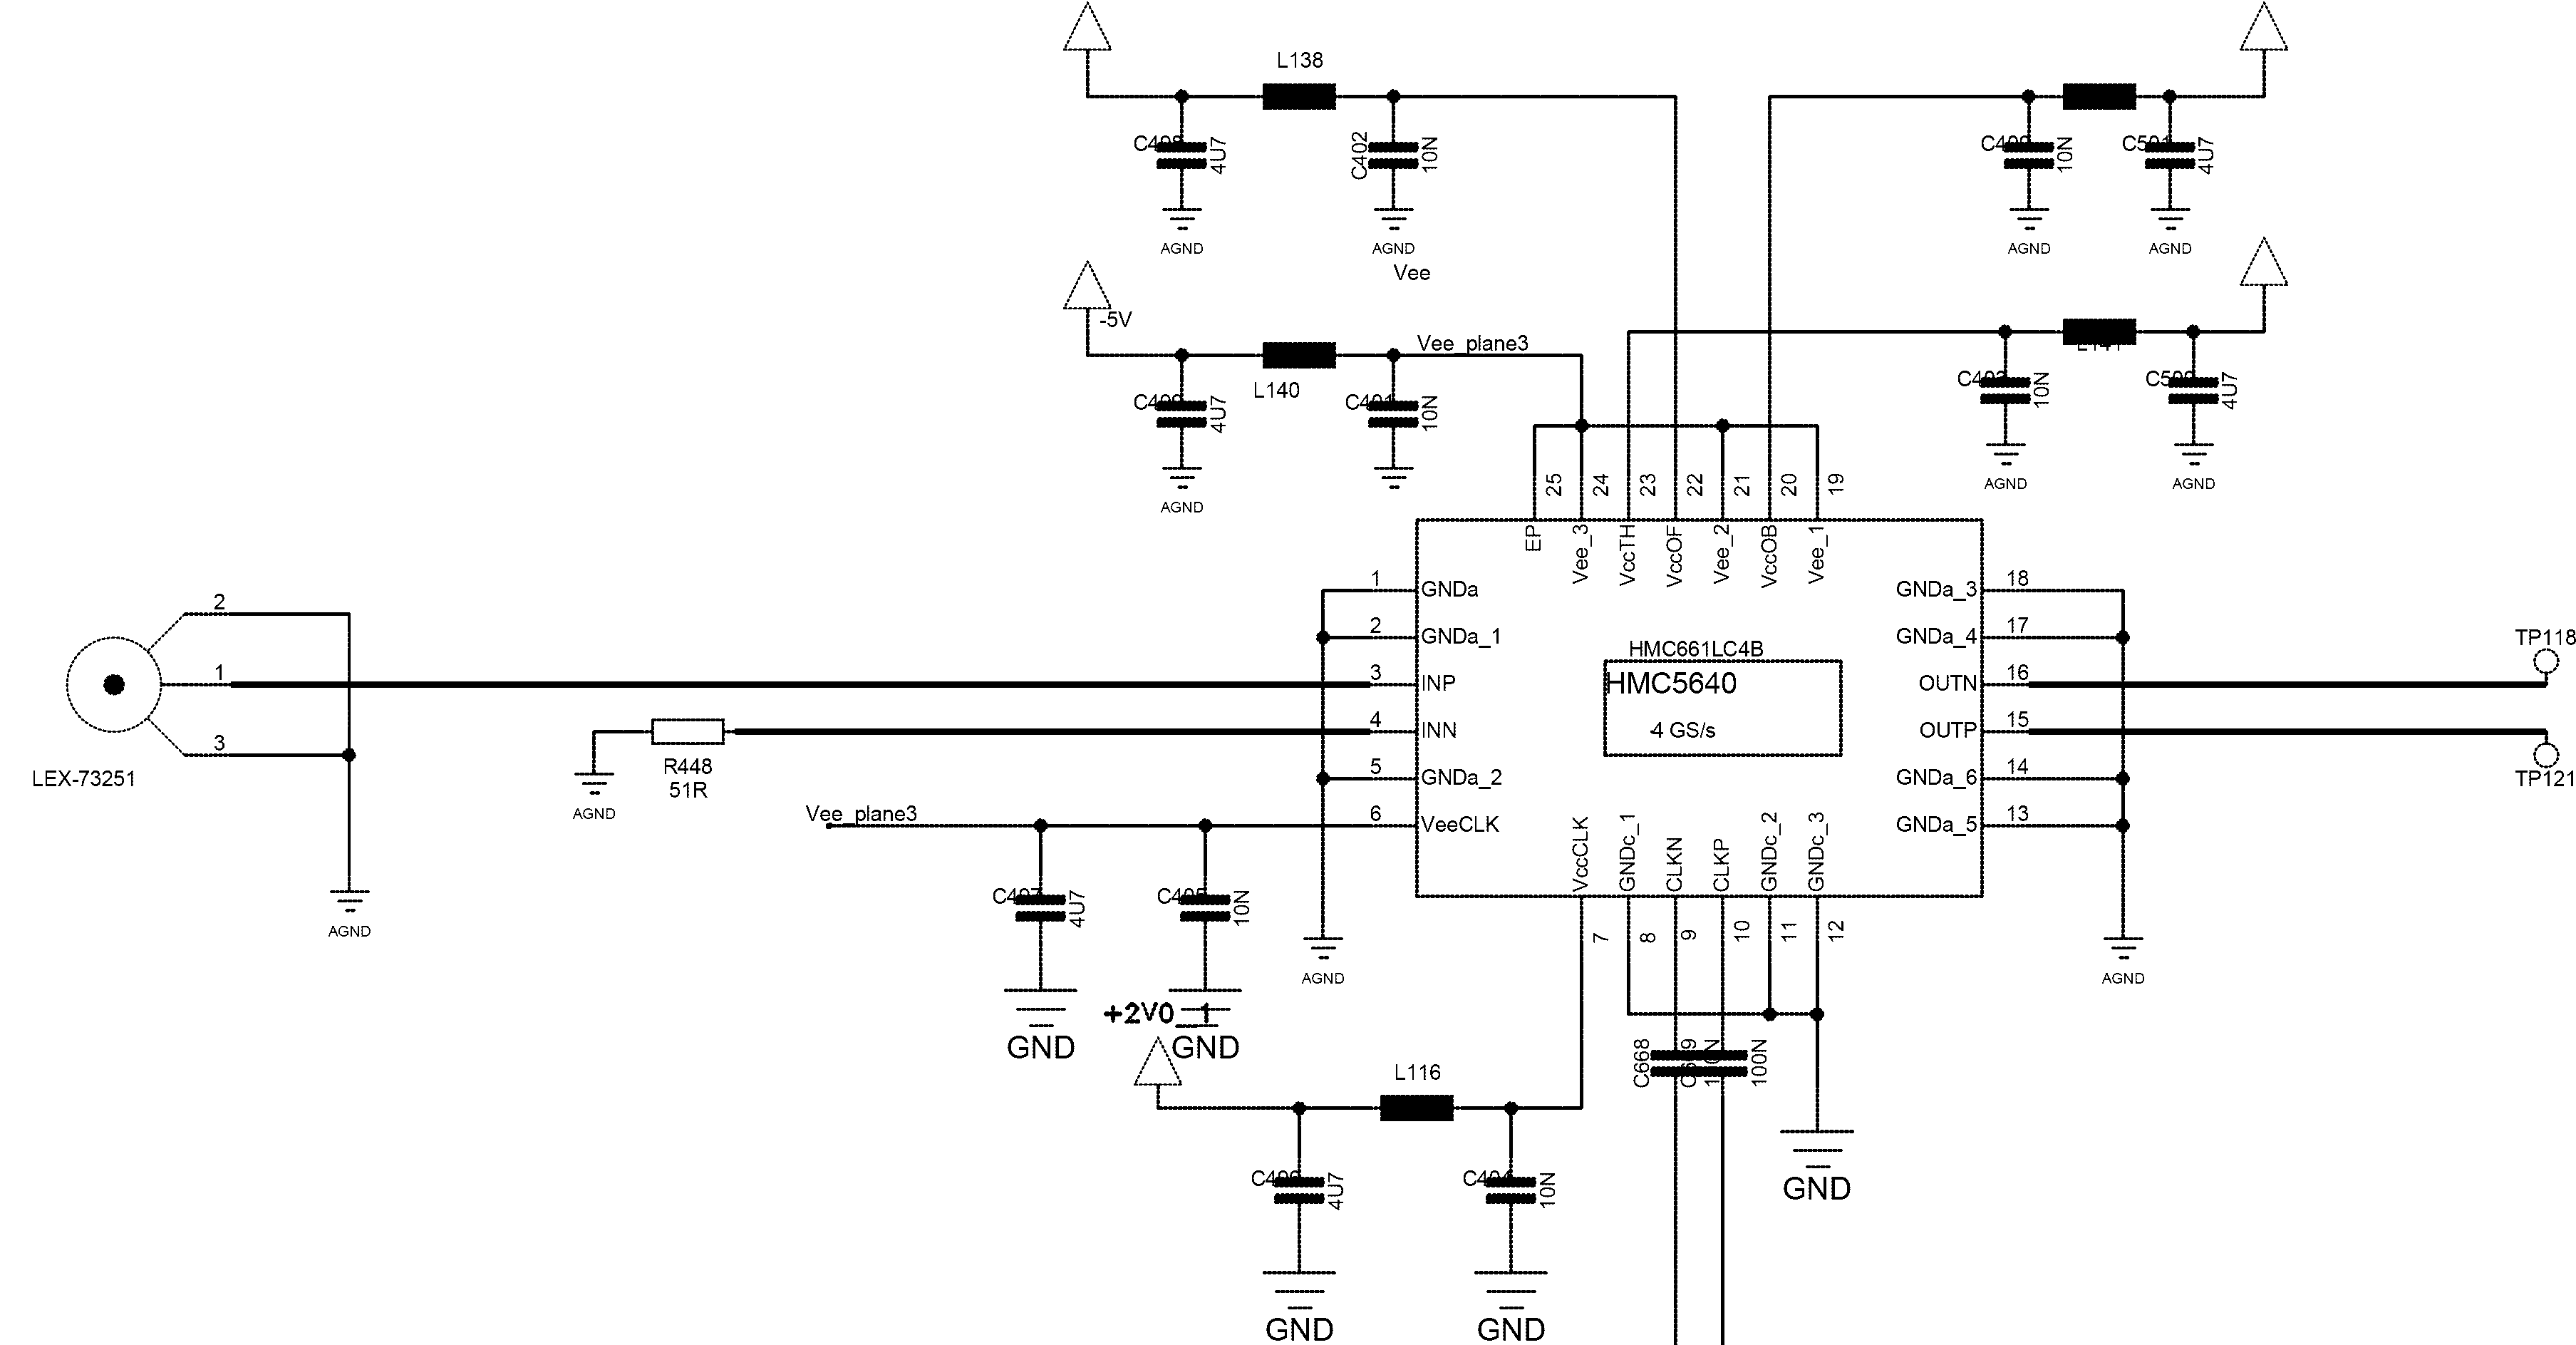
\includegraphics[width = \textwidth]{chap/04-work/img/hmc5640}
	\caption[HMC5640 THA schematic]{HMC5640 \gls{tha} schematic}
	\label{fig:hmc5640}
\end{figure}
%todo better picture/somehow improve this BS
%todo maybe only a pic of the component itself


\paragraph{Delay Chip}
The delay chip is used to create a delay in the clocking signal, which then goes to the \gls{tha} chip. For the selection of the delay chip, the most important characteristic, apart from jitter, is the delay step size and delay range. 

As indicated in \autoref{ssec:interl_impl}, the step-size of the delay chip must not exceed \SI{25}{\pico \second} to use the technique with \glspl{adc} sampling at \SI{2.5}{\giga \hertz}.

With the HMC856 programmable delay chip from \textit{Analog Devices}, which is also used for the \gls{kapture} sampling board, a minimal step size of \SI{3}{\pico\second} \cite{hmc856} is possible.
This is much less than  \SI{25}{\pico \second} and thus the chip could be potentially used for the intended purpose.
However, one drawback is the maximal delay range of \SI{100}{\pico\second}.
Considering a signal, which is stretched over several nanoseconds, this range limits the possibility to freely chose the overall timing resolution.
Another problem is the programming interface of the chip, which consists of five differential \gls{cml} inputs.
This means, one chip already takes up 10 pins only for control signals.
For in total 16 necessary delay chips, this results in 160 pins used only for control of the delay chips.
This occupies all pins of the \gls{fmc}+ connector (see \autoref{sec:connectors}) available for the user. 

A better candidate is the dual channel programmable delay chip NB6L295 from \textit{ON Semiconductor}. 
This chip provides two separately programmable delay channels. This has the benefit of reducing the total chip count by half, as now two \glspl{tha} can be connected to one delay chip.

The minimal delay step size of \SI{11}{\pico\second} lies under the maximal \SI{25}{\pico \second}. Therefore the chip is suitable for the targeted interleaving method, covering a total delay range from \SI{3.2}{\nano\second} to \SI{8.8}{\nano\second} per delay channel.

The chip is programmed via \gls{sdi}, which only requires 4 pins (enable pin, data pin, clock pin, load pin). %TODO maybe explain the pins more, don't know
Thus, the total number of digital control pins used by the delay chips is $4\cdot8 = 32$, which is a significant reduction compared to the 160 control pins needed by the HMC856 chips.
\begin{figure}[tbh]
	\centering
	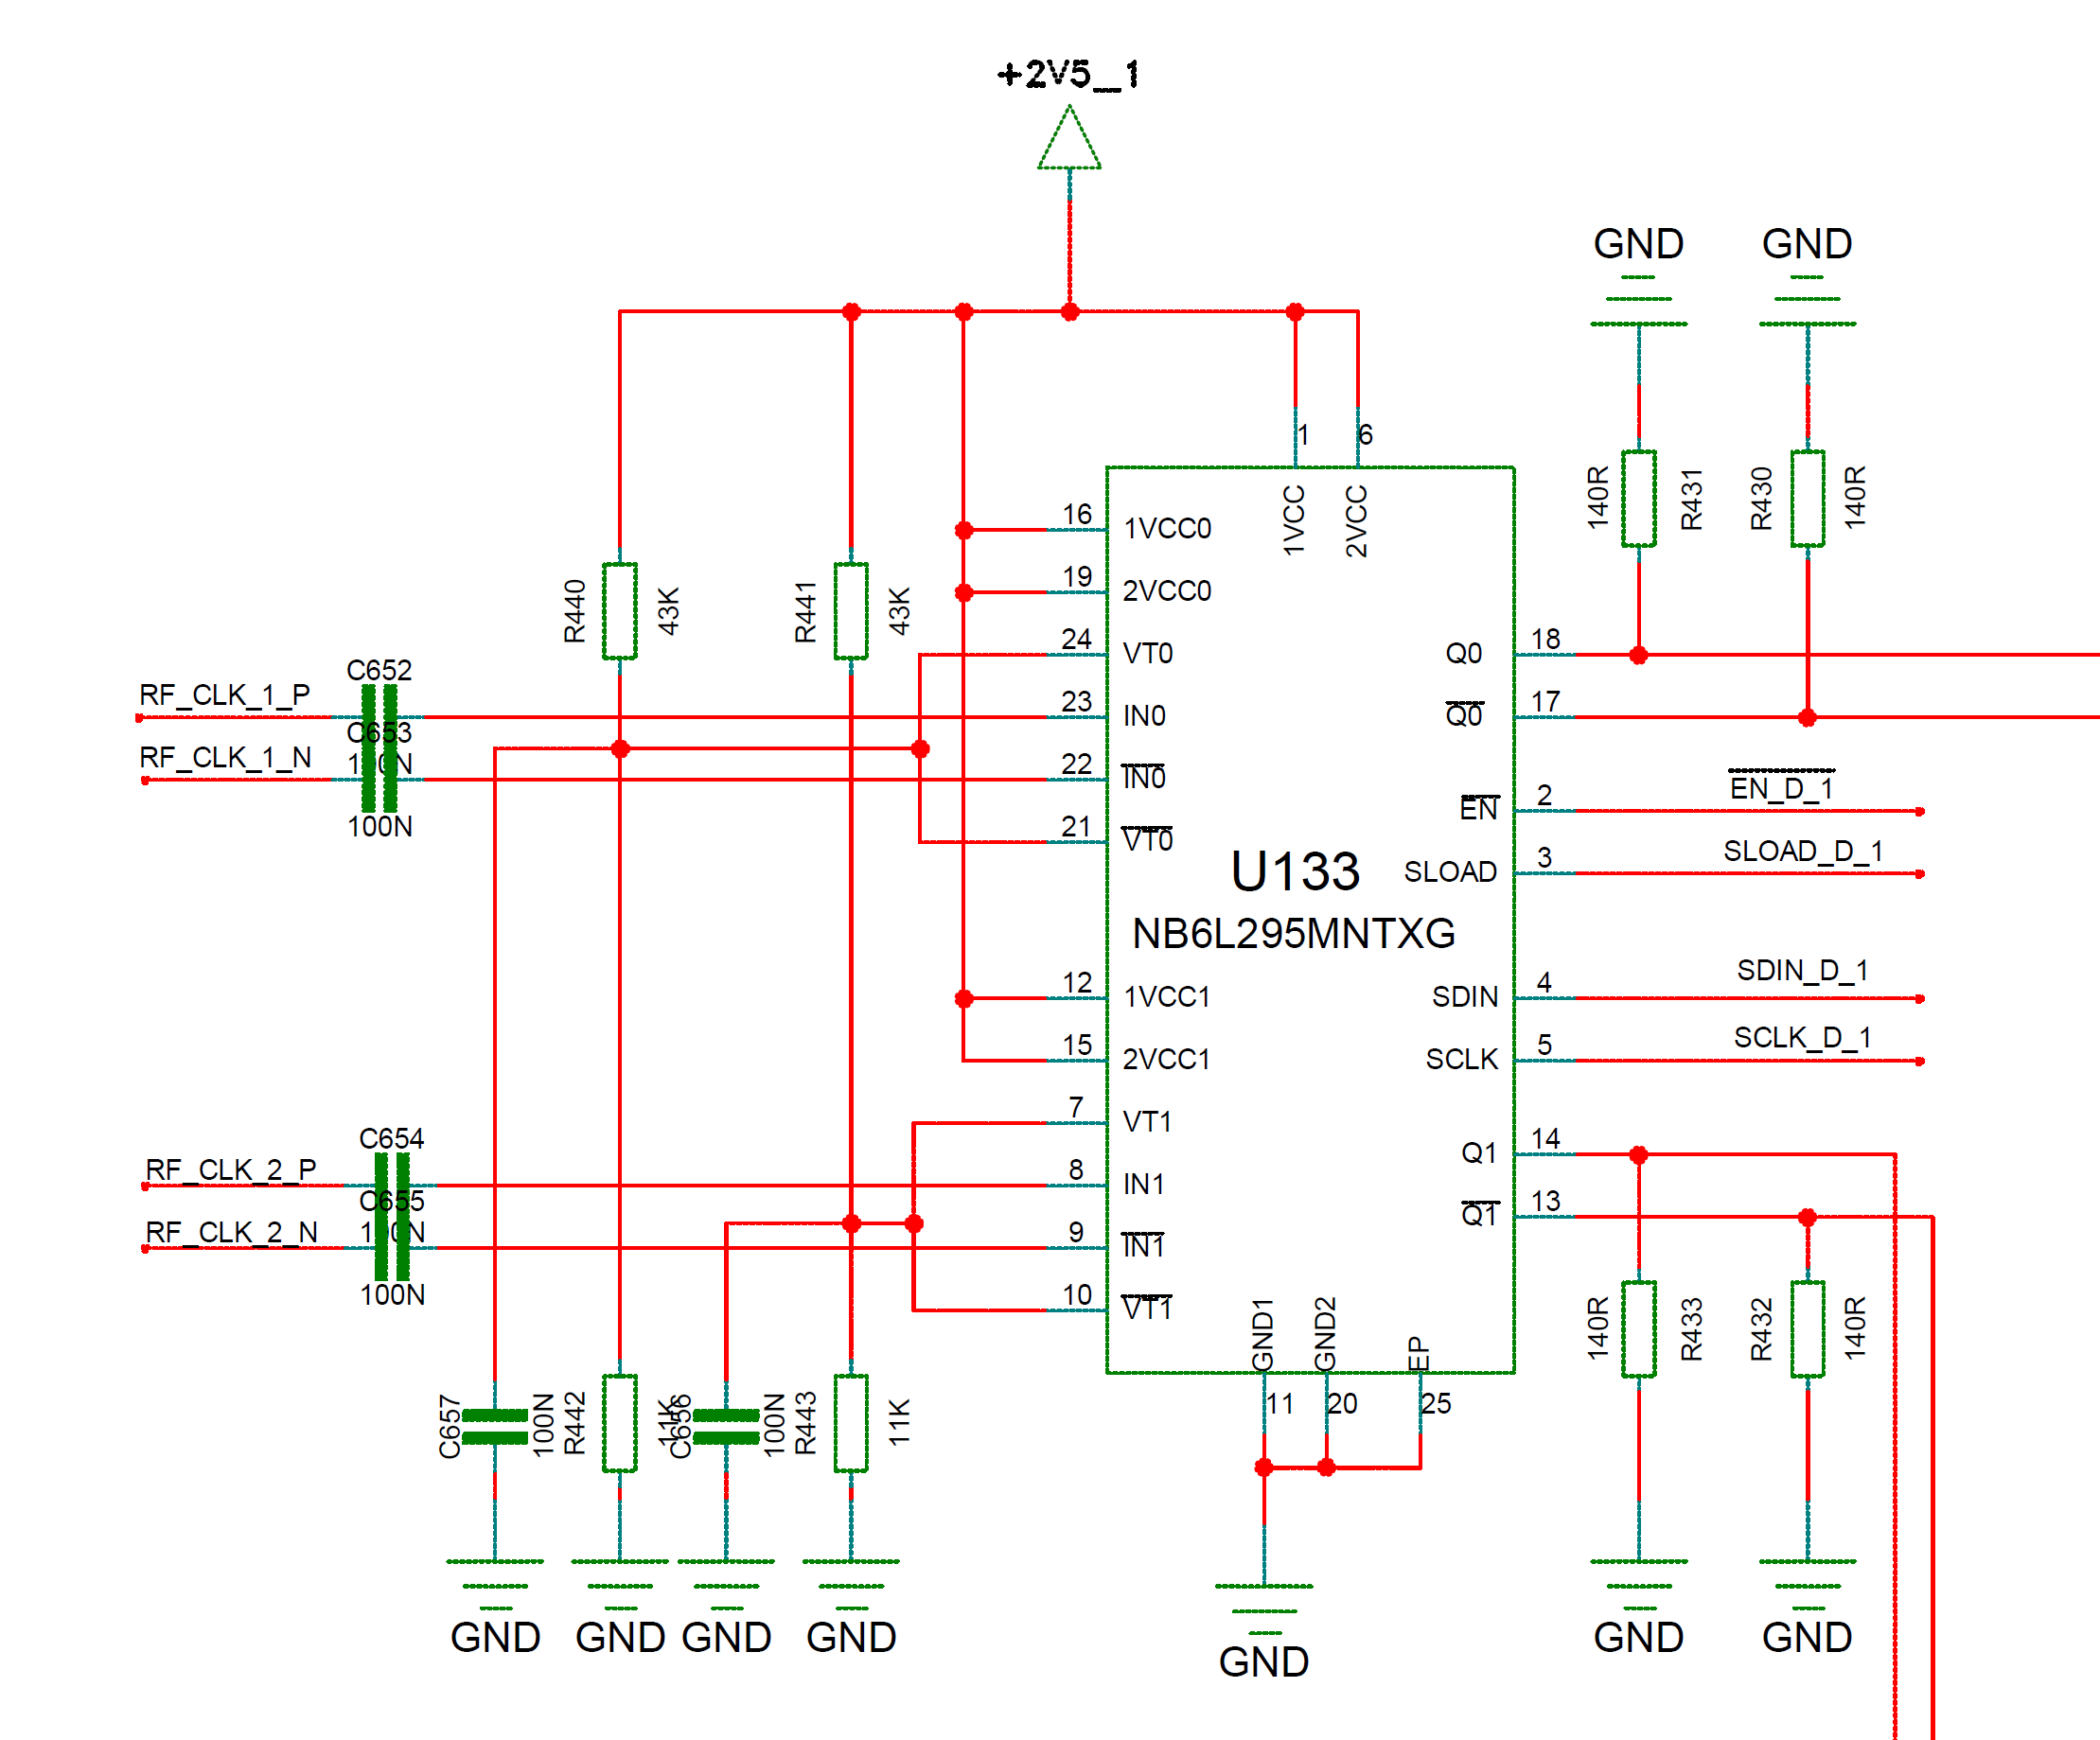
\includegraphics[width = \textwidth]{chap/04-work/img/delay_chip}
	\caption[NB6L295 delay chip schematic]{NB6L295 schematic}
	\label{fig:nb6l295}
\end{figure}


\paragraph{Inputs}
The inputs of the delay chip are driven by the preceding \gls{pll}, the outputs of which are \gls{lvpecl} drivers.
According to the data sheet, when driving the inputs with a \gls{lvpecl} driver, the VTx and $\overline{\text{VTx}}$ pins of the delay chip need to be connected to $V_\text{cc} - \SI{2}{\volt}$ (see \autoref{fig:delay_lvpecl}).
In case of $V_\text{cc}$ = \SI{2.5}{\volt}, this results in a voltage level of VTx = $\overline{\text{VTx}}$ = \SI{0.5}{\volt}.

To avoid using an additional voltage regulator, this voltage level is achieved by using a resistive voltage divider connected to $V_\text{cc}$.
Choosing the resistor values $\SI{43}{\kilo\ohm}$ and $\SI{11}{\kilo\ohm}$ results in a voltage of
\begin{equation}
	V_\text{cc} \frac{\SI{11}{\kilo\ohm}}{\SI{11}{\kilo\ohm} + \SI{43}{\kilo\ohm}} = \SI{0.5093}{\volt} \approx \SI{0.5}{\volt}
\end{equation}
%todo maybe give the circuit used with R1 and R2 or sth

A \SI{100}{\nano\farad} capacitor is put in parallel for power supply decoupling.

\begin{figure}[tbh]
	\centering
	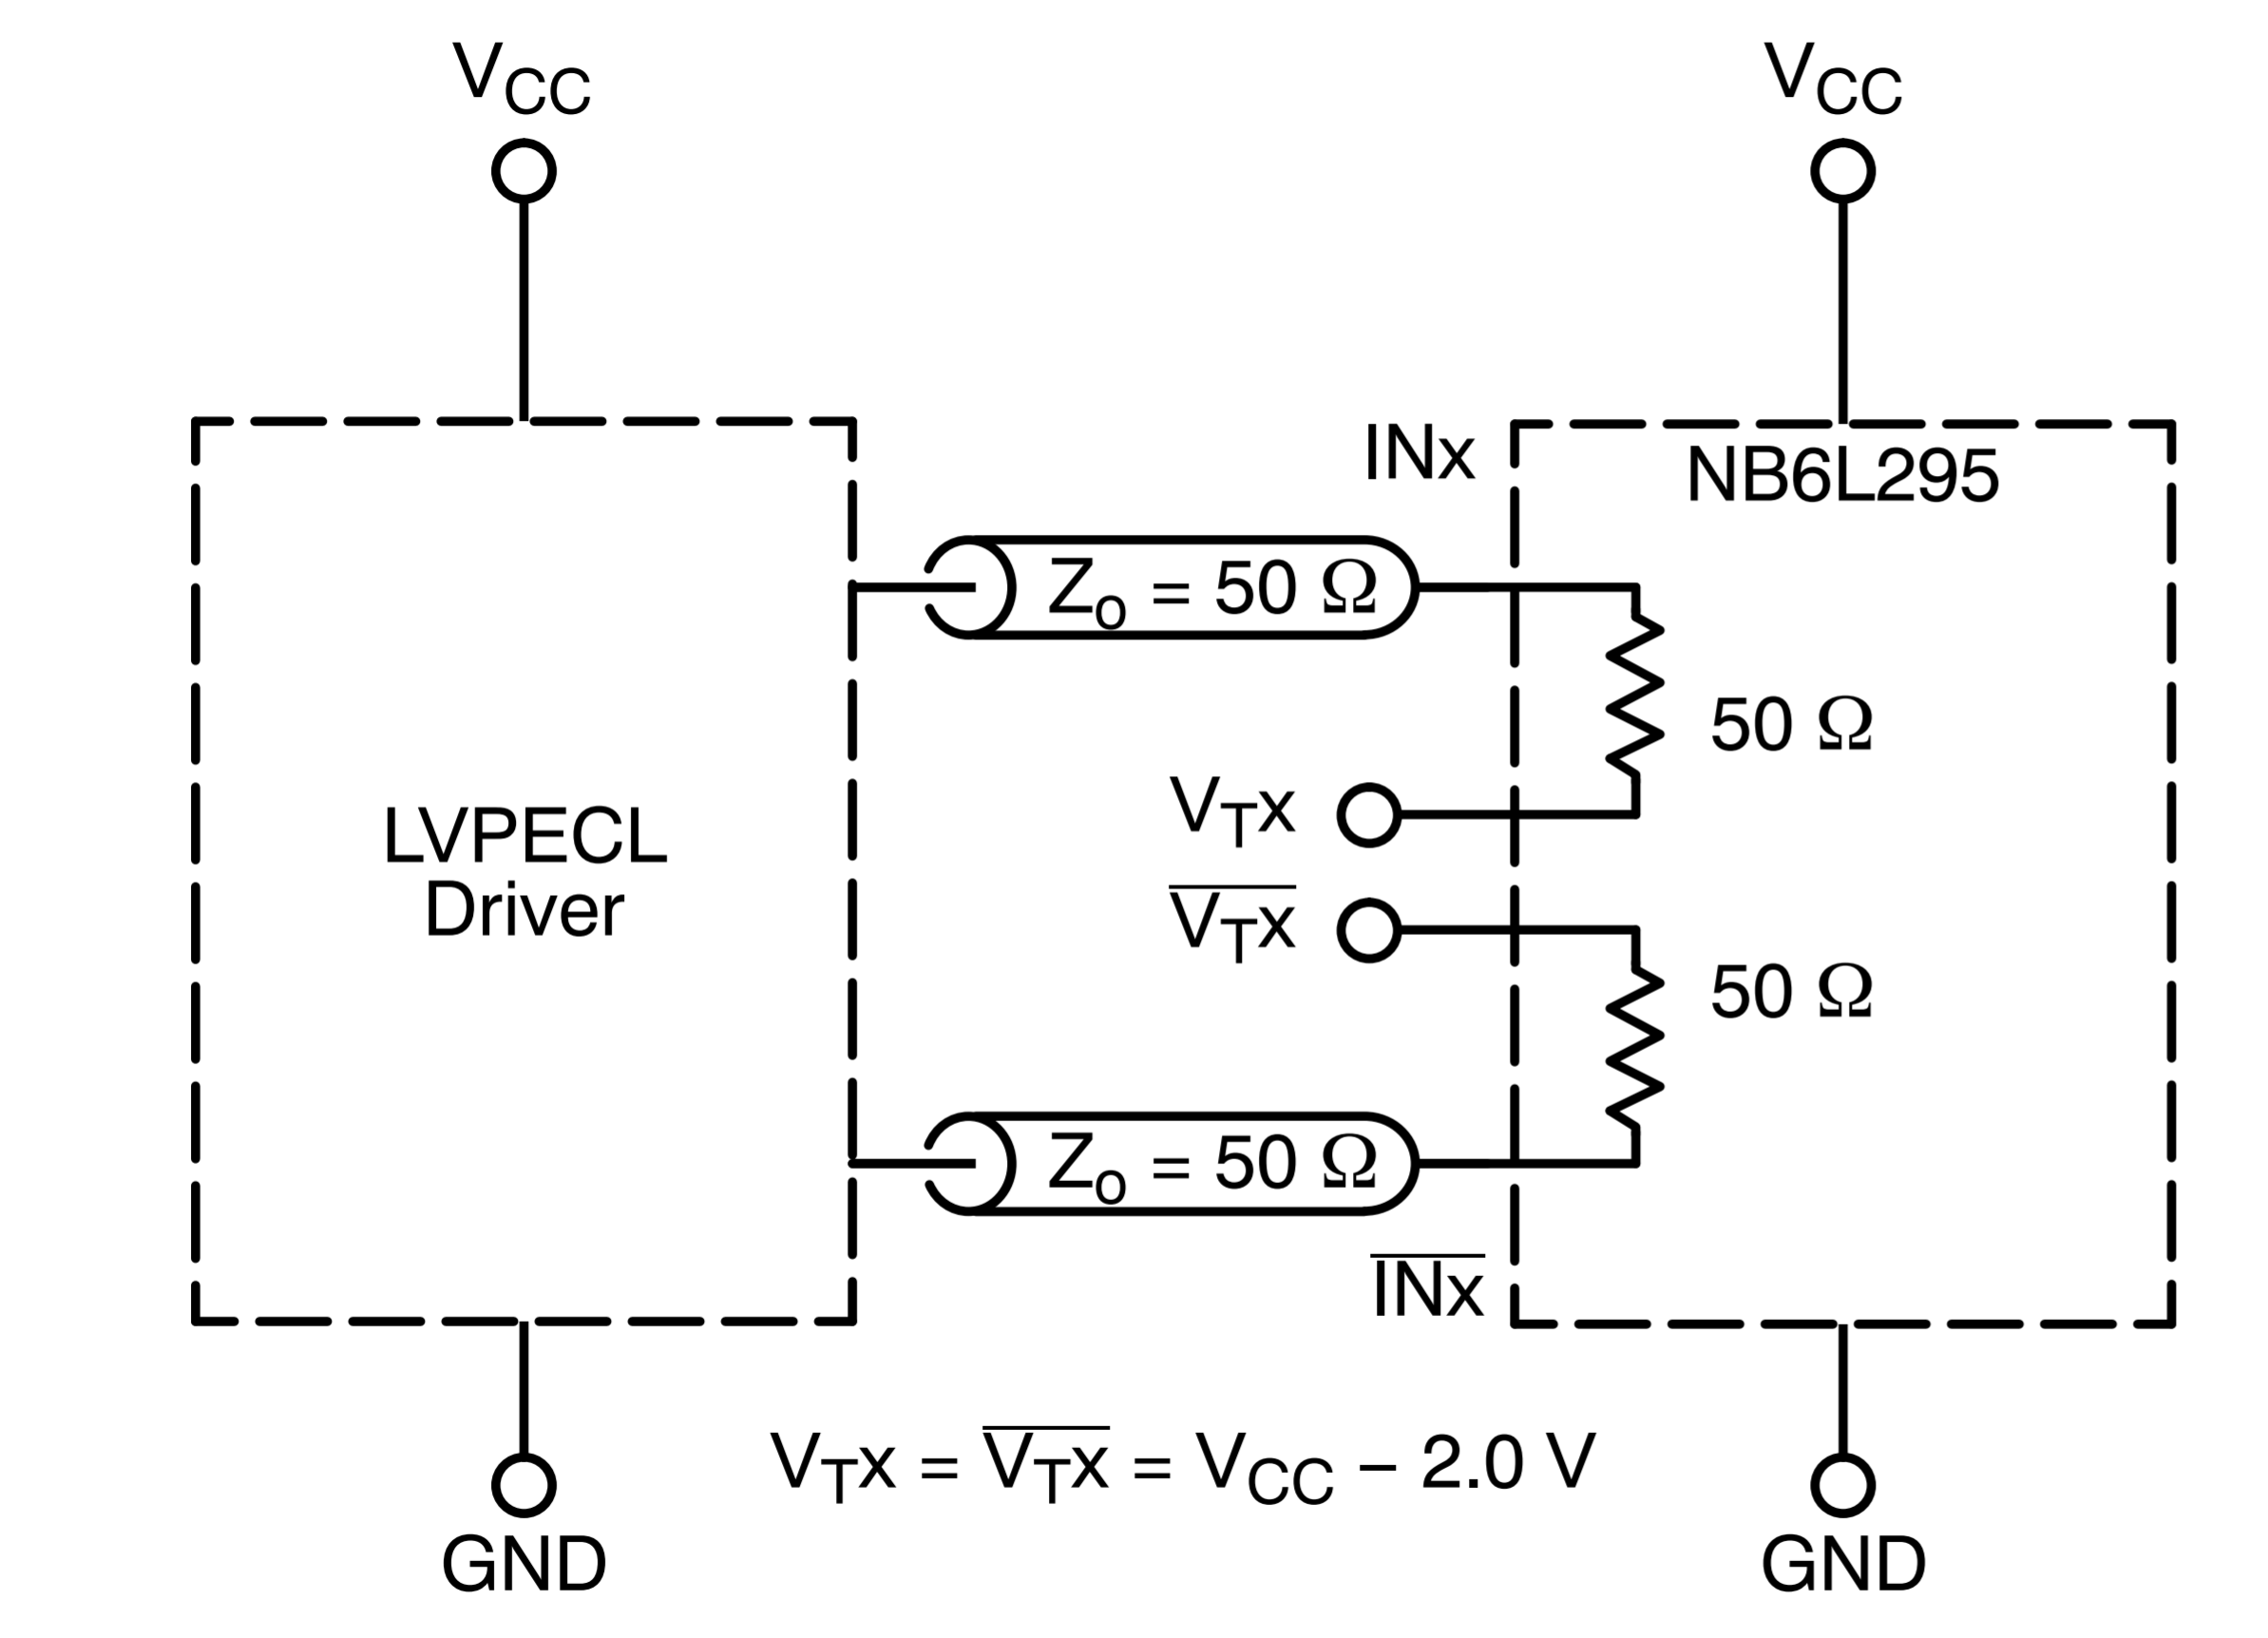
\includegraphics[width = 0.7\textwidth]{chap/04-work/img/delay_lvpecl}
	\caption[NB6L295 Delay Chip Schematic]{LVPECL recommendations for NB6L295 \cite{NB6L295}}
	\label{fig:delay_lvpecl}
\end{figure}


\begin{table}[tbh]
	\caption[NB6L295 Characteristics]{Specifications of the NB6L295 delay chip \cite{NB6L295}}
	\label{tab:nb6l295}
	\begin{minipage}{\textwidth}
		\centering
		\begin{tabularx}{\textwidth}{Xcccc}
			\toprule
			\textbf{Parameter} & \textbf{Min} & \textbf{Typ.} & \textbf{Max} & \textbf{Unit}\\
			\midrule
			\textbf{Outputs} &&&& \\
			Output HIGH Voltage & $V_{cc} - 1075$ & $V_{cc} - 950$ & $V_{cc} - 825$ & mV\\
			Output LOW Voltage & $V_{cc} - 1825$ & $V_{cc} - 1725$ & $V_{cc} - 1625$ & mV\\
			Common mode voltage & -0.1 & 0 & 0.1 & V\\[0.3cm]
			\textbf{AC Characteristics} &&&&\\
			Random Clock Jitter \gls{rms}&  & 3 & 10 & ps\\
			Output Rise/Fall Times (@\SI{50}{\mega \hertz}) & 85 & 120 & 170 & ps\\
			Serial Clock Input Frequency (50\% Duty Cycle\footnote{Percentage of the ratio of pulse width and total period of the waveform.}) &  &  & 20 & MHz\\
			Minimum Pulse width SLOAD  & 1 &  &  & ns\\
			\bottomrule
		\end{tabularx}
	\end{minipage}
\end{table}


\paragraph{Outputs}
The output of the delay chip is using a \gls{lvpecl} signaling interface, which is based on an open-emitter topology (see \autoref{fig:lvpecl}).
This requires a path to \gls{dc}, which is achieved by adding \SI{140}{\ohm} resistors.

\begin{figure}[tbh]
	\centering
	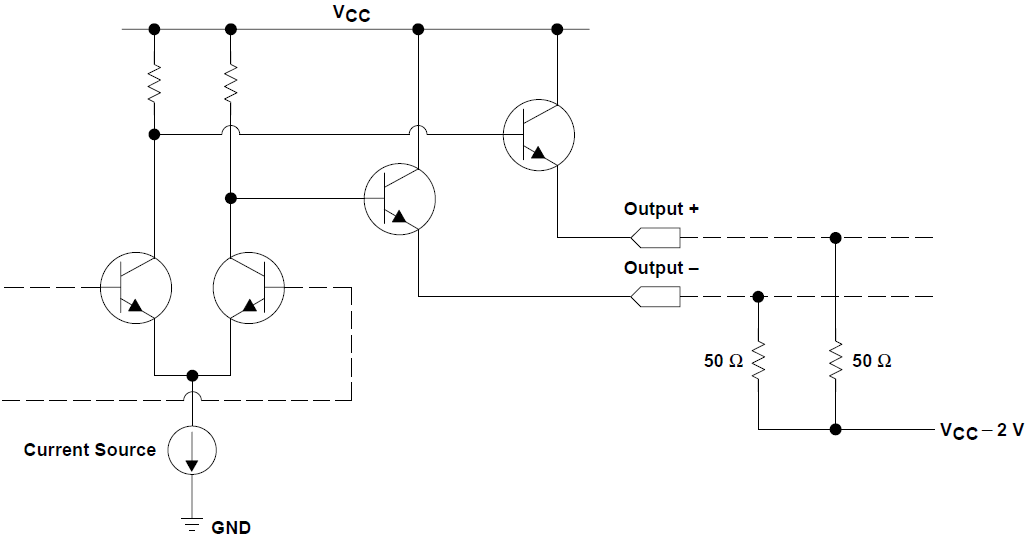
\includegraphics[width = \textwidth]{chap/04-work/img/lvpecl}
	\caption[LVPECL driver topology]{LVPECL driver topology. Left side shows the emitter-follower based driver. On the right, an example biasing with resistors is shown. \cite{lvpecl}}
	\label{fig:lvpecl}
\end{figure}
%TODO to tikz

As the output will be connected to the \gls{tha}, it is necessary to check the compatibility of the maximum amplitude and common-mode of the pins.

According to the data sheet \cite{NB6L295}, the voltage level of the output can vary between  $V_\text{cc} - \SI{1825}{\milli\volt}$ and $V_\text{cc} - \SI{825}{\milli\volt}$ (see \autoref{tab:nb6l295}).
Maximal voltage amplitude acceptable by the \gls{tha} inputs is \SI{2000}{\milli\volt} (see \autoref{tab:hmc5640}).
When using a supply voltage of $V_\text{cc} = \SI{3.3}{\volt}$, provided e.g. by the read-out card through the \gls{fmc}+ connector, this leads to a maximum output level of \SI{2475}{\milli\volt}.
This exceeds the limit given by the \gls{tha}.
Therefore, for $V_\text{cc}$ a smaller voltage should be considered.
In this design a voltage of $V_\text{cc} = \SI{2.5}{\volt}$ is chosen, which guarantees that the amplitude falls within the range \SIrange{675}{1675}{\milli\volt}.

The second point to consider is the common mode voltages. 
According to the data sheet of the \gls{tha}, the common mode voltage of the input clock pins is \SI{0.1}{\volt} (see \autoref{tab:hmc5640}).
The common mode voltage of the delay chip is not explicitly mentioned in the data sheet, thus it has to be calculated.
The common mode voltage $V_\text{CM}$ is just the mean value between the high level and the low level voltage of the output pins:
\begin{equation}
	V_\text{CM} = \frac{V_\text{out, LOW} + V_\text{out, HIGH}}{2}.
\end{equation}
According to this, the common mode voltage $V_{\text{CM}}$ of the delay chip output, when taking the minimum/maximum voltage level values, is 
\begin{equation}
	V_\text{CM} = \frac{\SI{675}{\milli \volt} + \SI{1675}{\milli \volt}}{2} = \SI{1175}{\milli \volt}.
\end{equation}
This is higher than the maximal input common mode voltage of the \gls{tha}.
\gls{ac} coupling is therefore necessary in this case.


%todo fix problem with [XSSSSS]
%todo parameters all caps, some capitalized, some not. choose one style

\subsection{Level Translator}
TODO

\subsection{Clock Distribution}
The clock distribution is designed as shown in \autoref{fig:clocking}.
\begin{figure}[tbh]
	\centering
	\includegraphics[width = \textwidth]{chap/04-work/img/pll_tsMode}
	\caption{Overview of the clocking paths on the sampling board}
	\label{fig:clocking}
\end{figure}
The LMK04808B low-noise clock jitter cleaner with dual-loop \glspl{pll} from \textit{Texas Instruments} cleans the incoming reference clock provided from the system (e.g. from \gls{kara}) for high temporal accuracy \cite{caselle2013}.
It is used with an external \gls{vcxo} from \textit{ABRACON}. 

The LMK04808B containts two \glspl{pll} (therefore called ``dual-loop''). 
The first \gls{pll} is used to clean the jitter from the reference clock. 
The second is then used to create a higher frequency clocking signal out of the cleaned clock. 

For proper functioning/best performance, a properly designed loop filter (see \autoref{fig:pll_block}) for both \glspl{pll} is needed. 
\textit{Texas Instruments} provides the \textit{PLLatinum Sim} tool, with which an appropriate loop filter can be calculated, given the device, desired loop bandwith, phase margin and frequency.
\begin{figure}[tbh]
	\centering
	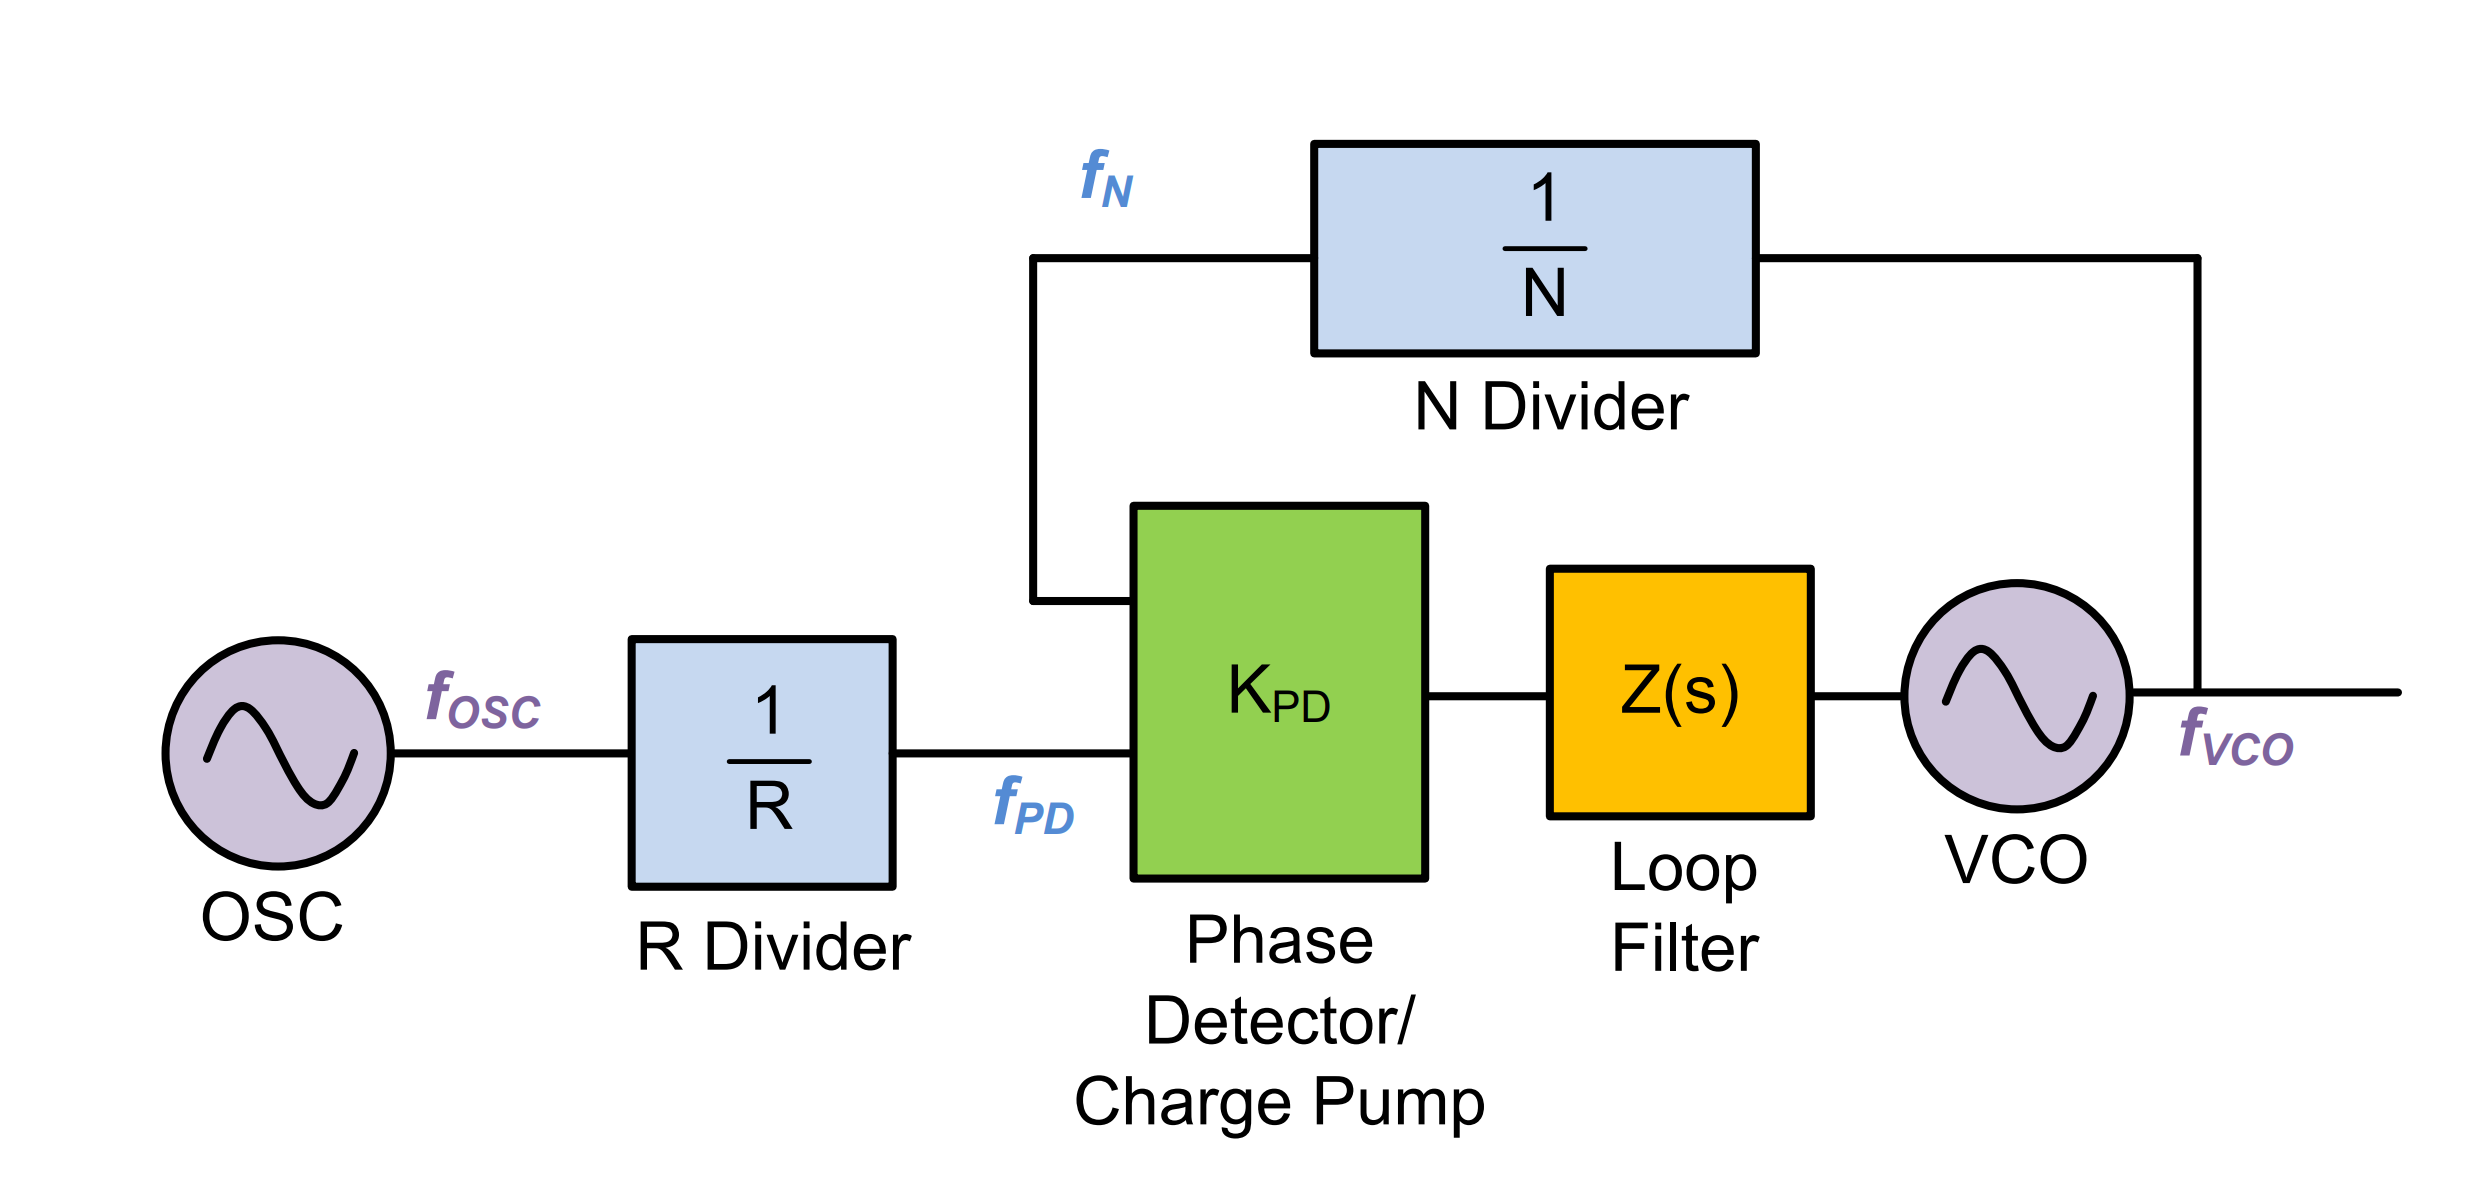
\includegraphics[width = \textwidth]{chap/04-work/img/pll_block}
	\caption[PLL block diagram]{General block diagram of a \gls{pll}}
	\label{fig:pll_block}
\end{figure}
The LMK04808B has only 12 outputs which is not enough for the 16 \glspl{tha} and additional clock signals needed for \gls{fpga}, \glspl{adc} and \gls{dac}. Furthermore, the outputs are divided into six groups à two outputs. 
Outputs in one group have the same configuration (frequency, phase, \ldots), which means that effectively only six different outputs are available.
Therefore, a low noise clock distribution fan-out buffer, the HMC987LP5E from \textit{Analog Devices}, is used for distributing the clock signal to the delay chips.
As one fan-out buffer has eight outputs, two chips are needed to cover all 16 channels. These chips get the output clock signal from two pins of the LMK04808B.
To ensure exactly identical clocking signals, both of the pins are chosen to be in one output group.
One output of the \gls{pll} is propagated to the \gls{fmc}+ connector as reference clock for the \gls{fpga}.
Up until this part, this clocking distribution architecture is not different from the one on the \gls{kapture} sampling board. 

As \autoref{fig:clocking} shows, the LMK04808B also provides a clocking signal to another \gls{pll}, the LMX2594 from \textit{Texas Instruments}.
The maximum output frequency of the LMK04808B is \SI{1536}{\mega \hertz}, not enough to clock the \glspl{adc} at maximum sampling rate (\SI{2.5}{\giga \sample \per \second}). 
A second \gls{pll} is therefore needed. 

The LMX2594 provides clocking signal frequencies up to \SI{15}{\giga \hertz} and is therefore a fitting candidate. 
To calculate the loop filter, the \textit{Texas Instruments} \textit{PLLatinum Sim} tool is used. The parameters of the used third order loop filter are as shown in \autoref{tab:lmx2594_filter}.
In order to provide the flexibility to enlarge the filter order, some of the components are considered in the schematics, but are either not placed or put to zero. 
In this way, a placeholder on the board is created.
The schematic of the LMX2594 is shown in \autoref{fig:lmx2594}.

Due to the \gls{adc} clocking limitations on the read-out card explained in \autoref{ssec:interl_impl}, two of the \glspl{pll} are needed. 
The reference clock signal is provided by outputs from different output groups of the LMK04808B. This way, the phase of each reference clock can be programmed individually, which allows to implement the \gls{adc} clocking technique described in \autoref{ssec:interl_impl}.


\begin{table}[tbh]
	\caption[LMX2594 Filter characteristics]{Filter characteristics}
	\label{tab:lmx2594_filter}
	\centering
	\begin{tabularx}{\textwidth}{Xl}
		\toprule
		\textbf{Parameter}                         & \textbf{Value}             \\ \bottomrule
		VCO Gain                                   & \SI{239}{\MHz\per\volt}    \\
		Loop Bandwidth                             & \SI{32.7}{\kHz}            \\
		Phase Margin                               & \ang{69}                   \\
		Effective Charge Pump Gain                 & \SI{3}{\milli\ampere}      \\
		Phase Detector Frequency                   & \SI{24.576}{\MHz}          \\
		VCXO Frequency                             & Designed for \SI{15}{\GHz} \\
		[0.3cm]
		 \textbf{Loop filter components} &                            \\
		$C_{1,\text{LF}}$                          & \SI{2200}{\pico\farad}     \\
		$C_{2,\text{LF}}$                          & \SI{180}{\nano\farad}      \\
		$C_{3,\text{LF}}$                          & \SI{1800}{\pico\farad}     \\
		$R_{2}$                                    & \SI{160}{\ohm}             \\
		$R_{3,\text{LF}}$                          & \SI{180}{\ohm}             \\ \bottomrule
	\end{tabularx}
\end{table}

\begin{figure}[tbh]
	\centering
	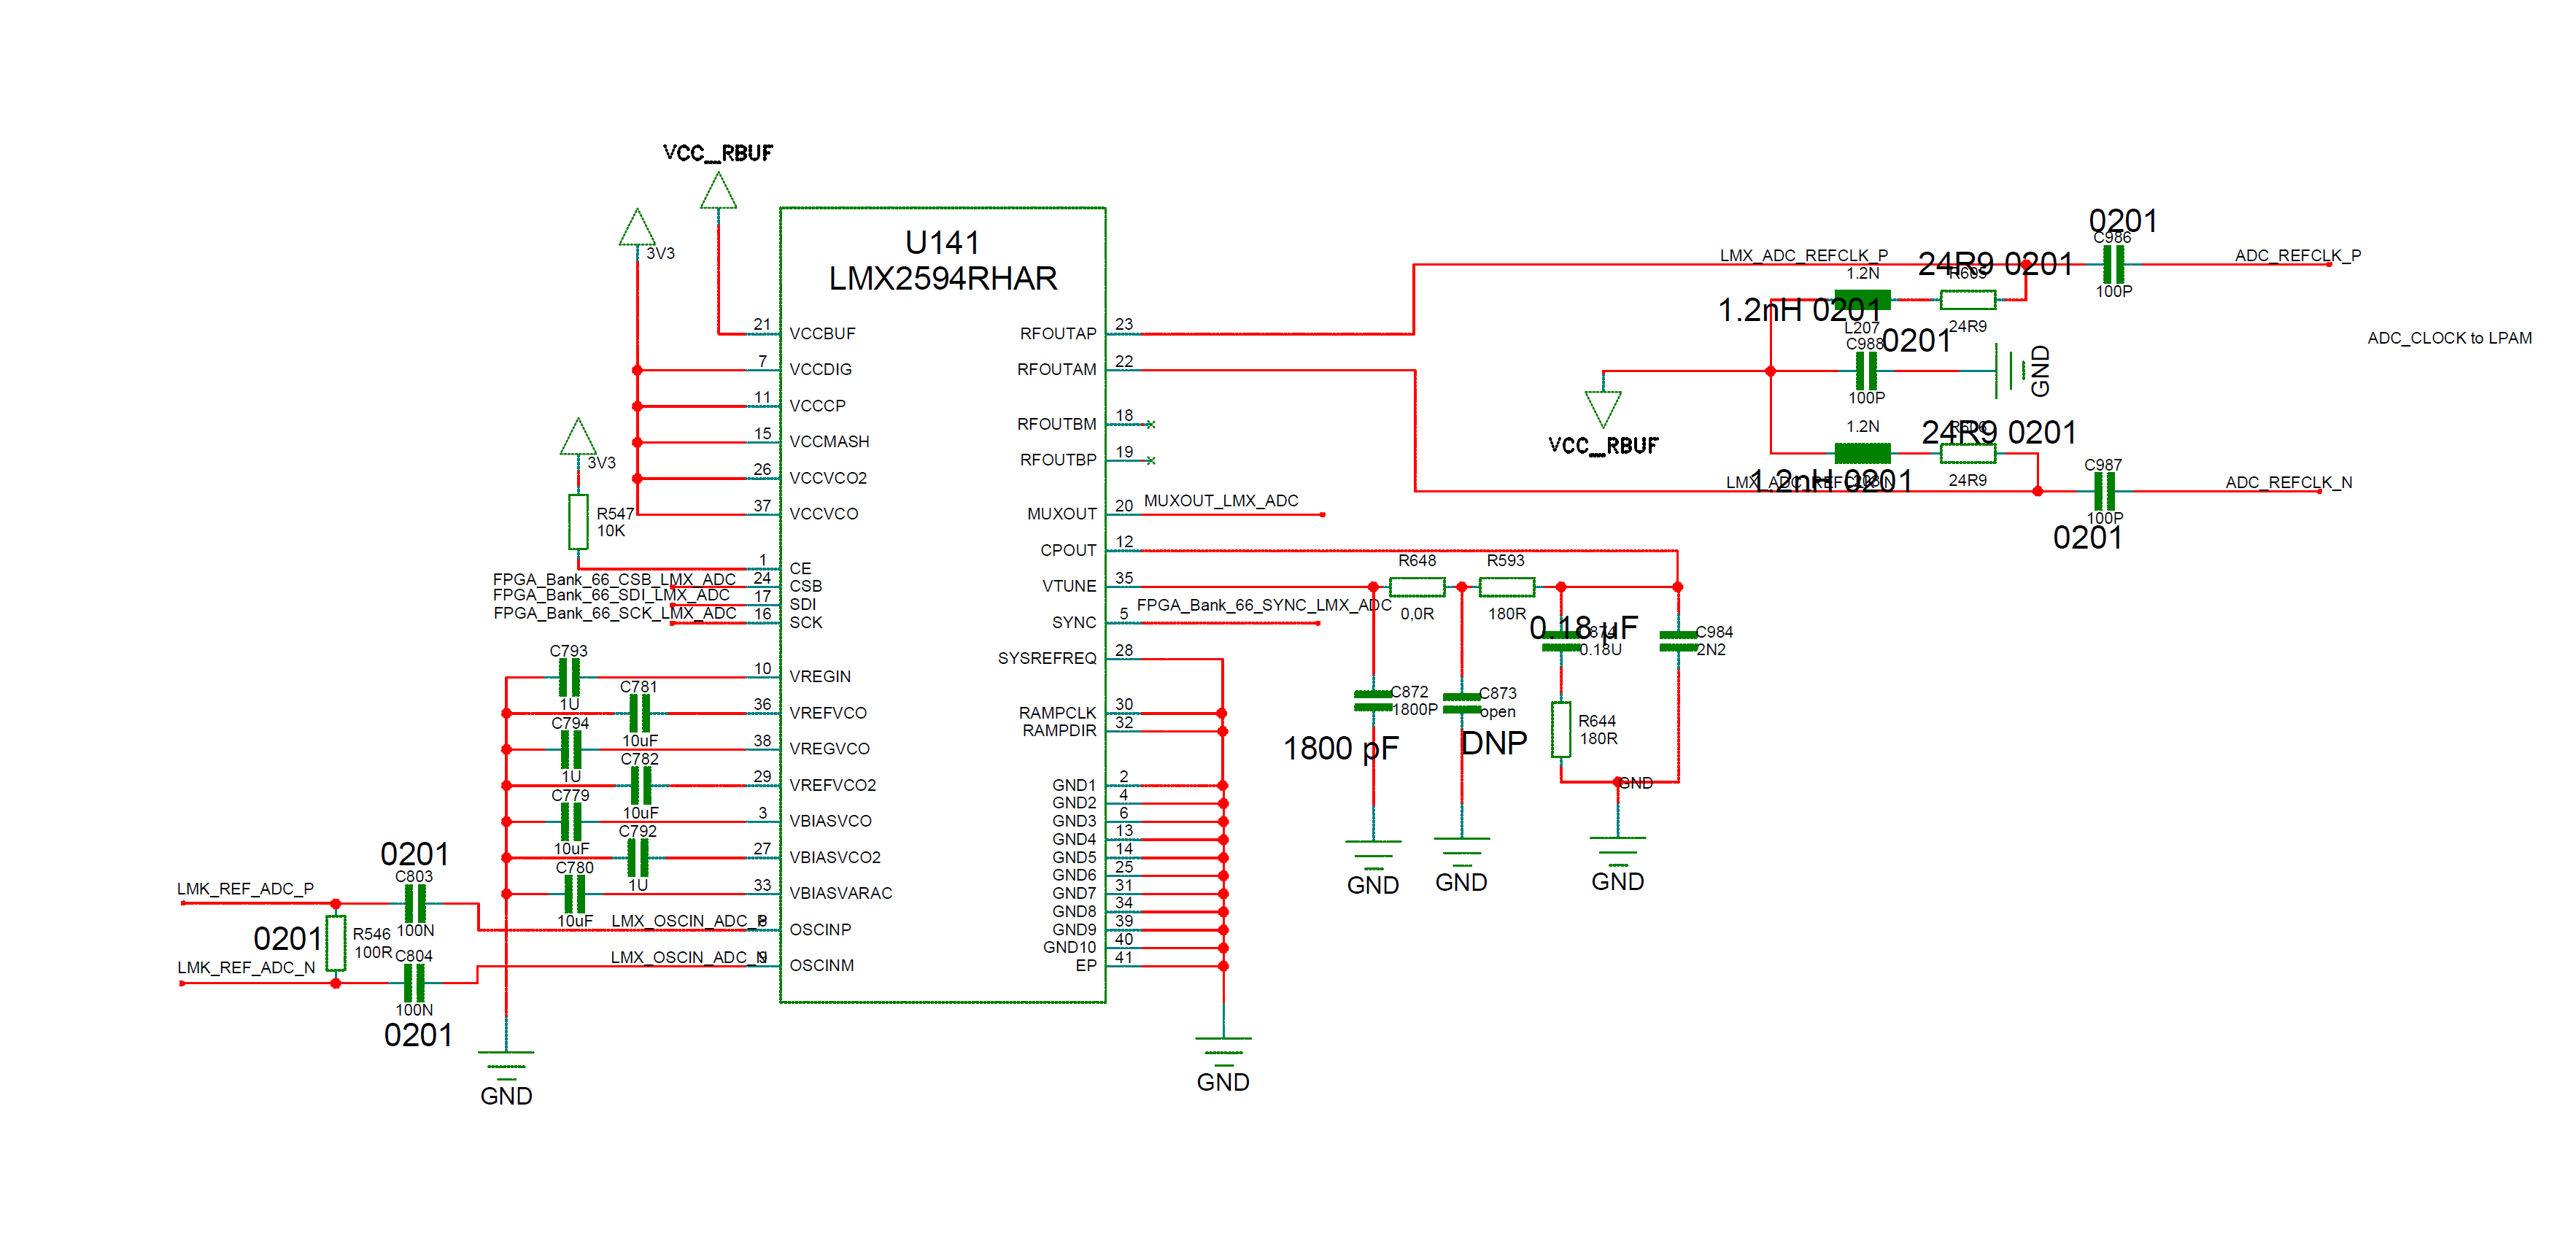
\includegraphics[width = \textwidth]{chap/04-work/img/lmx2594}
	\caption{Schematics of the LMX2594}
	\label{fig:lmx2594}
\end{figure}

 



\subsection{Digital-To-Analog-Converter Channels}
For test purposes, two \gls{dac} channels from the read-out card are routed on the sampling board.
In this way, test signals can be generated right on the read-out card, without the need for an external signal generator. 
The differential inputs from the \glspl{dac} are transformed into single ended outputs with dedicated baluns\footnote{\textbf{bal}anced to \textbf{un}balanced}. the BD3150N50100AHFa and the BD4859N50100AHF from \textit{Anaren}. These are used for the signal frequency range \SIrange{3.1}{5.0}{\GHz} and \SIrange{4.8}{5.9}{\GHz} respectively.

The single-ended output is connected to a miniature \gls{rf} connector from \textit{Hirose Electric}.

The schematic of a \gls{dac} channel is shown in \autoref{fig:dac_channel}.
\begin{figure}[tbh]
	\centering
	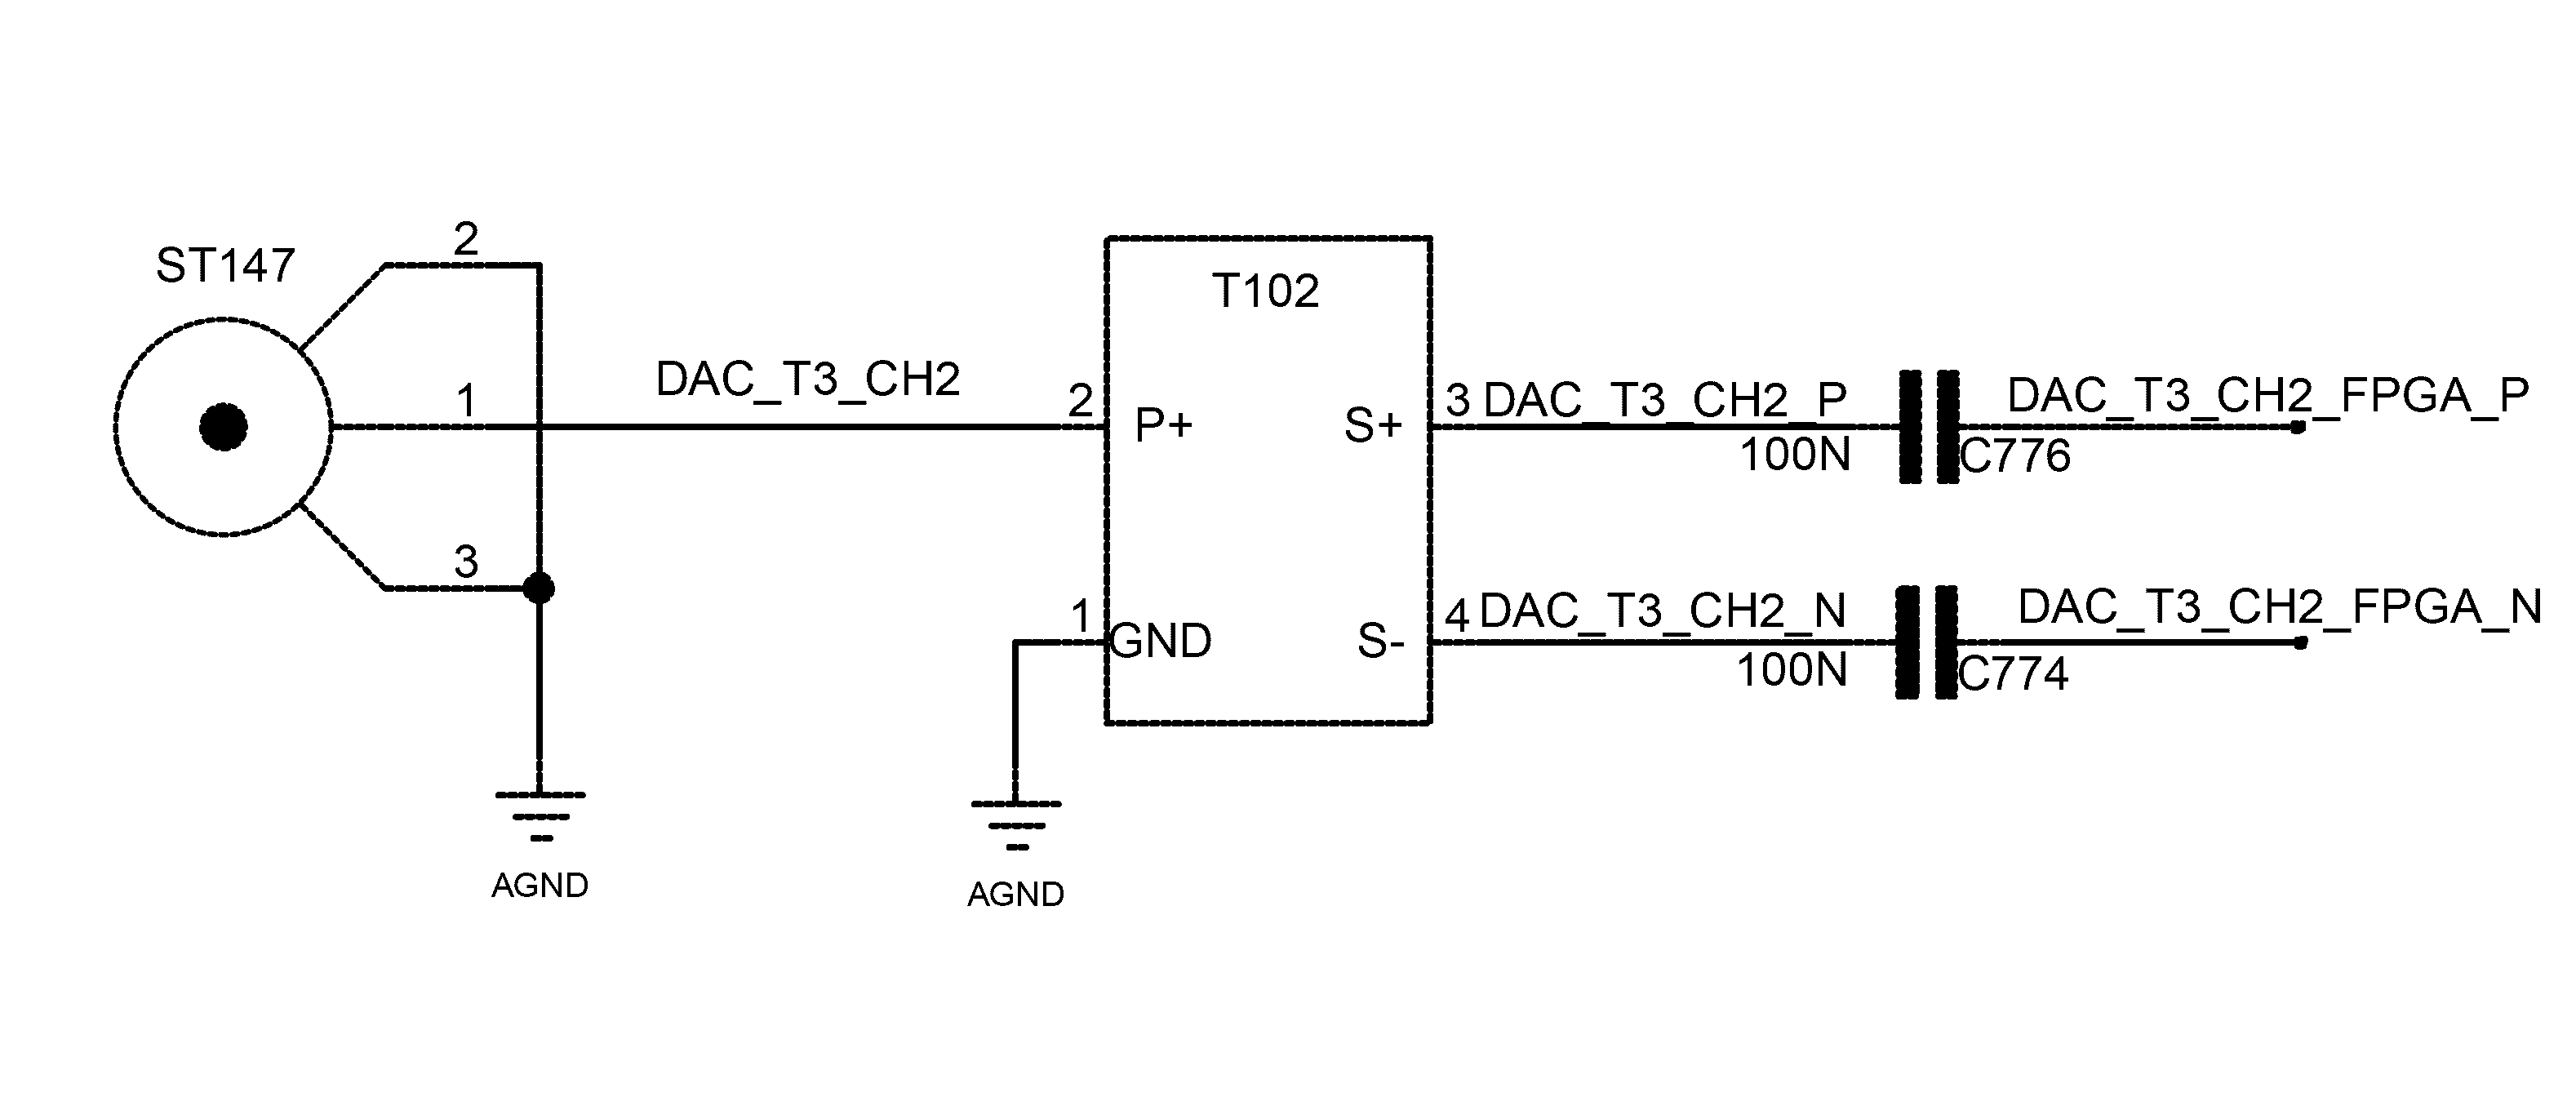
\includegraphics[width = \textwidth]{chap/04-work/img/dac_channel}
	\caption{DAC-channel with balun. Signal propagates from right to left.}
	\label{fig:dac_channel}
\end{figure}


\subsection{Power Supply}
Stable power supply is the key for best performance of the components. Especially high-performance \Glspl{ic}, such as \glspl{tha}, highly rely on a stable voltage level for correct functionality. 
Therefore, proper power supply design is an important step which needs to be handled with care.
This step includes choosing the right type and amount of voltage regulators, as well as providing appropriate filtering. 

\autoref{tab:theresacomp} lists the power supply requirements of all the components used on the board.

\begin{table}[tbh]
	\caption{Power consumption of components on the board}
	\label{tab:theresacomp}
	\begin{minipage}{\textwidth}
		\centering
		\begin{tabularx}{\textwidth}{Xlllll}
			\toprule
			\textbf{Component}          & $V_\text{cc}$ (V) & $I_\text{max}$ (A)                        & $P_\text{max}$ (W) & $\#_\text{parts}$ & $I_\text{tot}$\footnote{for 16 \glspl{adc}} (A) \\ \midrule
			HMC5649 (\gls{tha})          & 2                 & 0.221                                     & 0.442              & 16                & 3.536                                           \\
			                            & -5                & -0.242                                    & 1.21               &                   & 3.872                                           \\
			NB6L295 (Delay chip)              & 2.5              & 0.170                                     & 0.425 & 8                & 1.36                                            \\
			HMC987LP5E (Fanout buffer) & 3.3               & 0.234\footnote{All Outputs and RF-Buffer} & 0.772              & 2                 & 0.468                                           \\
			LMK04808B (\gls{pll})          & 3.3               & 0.590\footnote{All CLKs}                  & 1.947              & 1                 & 0.590                                         \\
			LMX2594 (\gls{pll})          & 3.3               & 0.340                & 1.122             & 2                 & 2.244 \\
			VCXO                        & 3.3               & 0.03                                      & 0.198              & 1                 & 0.03                                            \\ \bottomrule
		\end{tabularx}
	\end{minipage}
\end{table}
%todo why two rows for the HMC THA. what are the upper/lower values?
For general components, there are two power supply sources
\begin{itemize}
\item Voltage coming from FMC+ connector
\item External power supplies (-5V)
\end{itemize}
An EMI filter needs to be placed in order to keep noise of the power supply and read-out card from the sampling board.
This is not stable enough for the sensitive THA, therefore voltage regulators are needed.
These are able to regulate the voltage to be stable.


\paragraph{Power Supply for Track-and-Hold-Amplifiers}
The \glspl{tha} need a constant voltage level for optimal operation. To guarantee a stable voltage level, linear voltage regulators which are capable to maintain a stable output voltage, are to be used with the \glspl{tha}.

On the \gls{kapture} sampling board, the \gls{ldo} ADP1708 from \textit{Analog Devices} is used to provide a power supply for the \glspl{tha}. A \gls{ldo} is able to operate at a low potential difference between the input and output voltage. This low potential difference has also the benefit of low power dissipation, which also    
This power supply can provide at maximum \SI{1}{\ampere} to the load. 
In order to minimize the amount of components needed on the board, i.e. to save space, a component which can provide higher currents should be used. 
This way, one single voltage regulator can be used for more components.

For the new board, the ADP1741 low-dropout voltage regulator from \textit{Analog Devices} is used. This voltage regulator has adjustable output voltage from \SIrange{1.6}{3.6}{\volt} and a maximum output current of \SI{2}{\ampere}. 

With the given characteristics, it is now necessary to think about the amount of voltage regulators needed.
As a rule of thumb, the power supply should provide twice the maximum power needed by the components it drives. \cite{michele}
The power consumption/maximum current for the respective components on the sampling board is listed in \autoref{tab:kapturecomp}. 

It is necessary to think about the amount of voltage regulators needed. As a rule of thumb, the power supply should provide twice the maximum current (i.e. power) needed by the components it drives. \cite{michele} The power consumption/maximum current for the \glspl{tha} on is listed in \autoref{tab:kapturecomp}. 

The maximal current which the ADP1741 can provide @\SI{2}{\volt} is \SI{2}{\ampere}.
This means, with one \gls{tha} amplifier requiring a maximal current of \SI{0.221}{\ampere}, one ADP1741 can handle four units according to the rule mentioned beforehand:

\begin{align}
I_\text{max,ADP1741} &= \SI{2}{\ampere} > 2 * I_\text{tot}\\
I_\text{tot} &= 4 \cdot \SI{0.221}{\ampere} =  \SI{0.884}{\ampere}
\end{align}

\paragraph{Delay Chips}
The delay chips require \SI{2.5}{\volt}. They carry sensitive clock signals, therefore also needs stable voltage levels. 
Two other voltage regulators are used, they are an easy way to generate the voltage and keep it stable.
Two chips because of max. current draw from the chips.

\section{Layout}
The next step after schematic capture is the design of the layout.
In this step, the board outline (``form'') is defined, the components are placed and traces between them are routed.
\begin{itemize}
\item Define layer number
\item Choose substrate 
\item Calculate transmission line geometries for high frequency signals
\item Place components following proper decoupling techniques
\item Route traces, taking care that traces of the same group have same length. For sensitive signals take care that these are shielded by ground planes on the layers above and below.
\item Places additional structures to reduce cross-talk, EMI, etc. (via fences, stitching vias)
\item Create proper power distribution by placing copper planes at appropriate places.
\end{itemize}

For better understanding, first a general overview over \gls{pcb} structures is given. 
Then the steps mentioned above are described.
\subsection{PCB Structures Overview} \label{ssec:pcb_structs}
In this sectoin an overview over the basic structures on a \gls{pcb} is given.

\paragraph{Traces}
A \textit{trace} is a strip of metal, which establishes an electrical connection and carries signals between two (or more) points in the horizontal plane of a \gls{pcb}. \cite{xilDecouple}


\paragraph{Planes}
\textit{Plane} denotes an uninterrupted area of metal, which covers the whole \gls{pcb} layer. If this area only covers a part of the layer, it is called a \textit{planelet}. These areas provide power distribution across the \gls{pcb} and present an important transmission medium for the return current\footnote{Any current, which is injected into the components/boards, needs a return path, as otherwise there is no closed circuit.}. \cite{xilDecouple}

\paragraph{Vias}
A via is metal-plated hole, which is used to route a trace in vertical direction, i.e. from the \gls{pcb} outer layer to the inner layers. They carry signals and power. Three types of vias are \cite{vias}:
\begin{itemize}
	\item Blind via: A blind via connects the surface layers with at most three layers below.
	\item Buried via: A buried via only connects internal layers.
	\item Through via: A through via goes from one \gls{pcb} surface to another and is used to connect any layer. 
\end{itemize}
\begin{figure}[tbh]
	\centering
	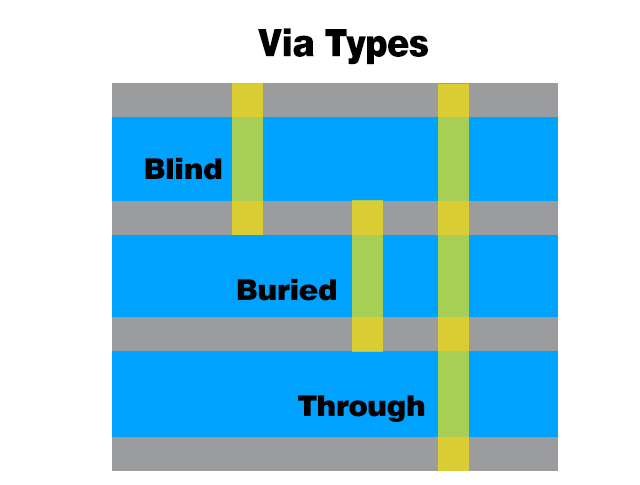
\includegraphics[width = 0.7\textwidth]{chap/04-work/img/vias}
	\caption[Via types]{Visualization of via types \cite{vias}}
	\label{fig:vias}
\end{figure}
\textbf{TODO:} 
	\begin{itemize}
		\item Via fences
		\item Pads
	\end{itemize}
%todo bild

In this design only blind and through vias are used.

\subsection{\gls{pcb} Substrate Selection and Stackup}
Proper substrate material has to be selected in according to the use-case.
The MEGTRON 6 from \textit{Panasonic} is designed for high-speed/high frequency applications. 
Characteristics of this material are:
\begin{itemize}
\item Low dielectric constant: $\epsilon_r$ = 3.61 at \SI{10}{\giga \hertz}, 3.71 at \SI{1}{\giga \hertz}
\item Low dielectric dissipation factor: 0.002 at \SI{10}{\giga \hertz}, 0.004 at \SI{1}{\giga \hertz}
\item Low transmission loss
\item High heat resistance: Decomposition temperature $T_d$ = \SI{410}{\celsius}
\end{itemize}

Another important step is deciding the number of layers. The complexity of the board implies that a lot of layers are needed, for this design 16.

\begin{figure}[tbh]
	\centering
	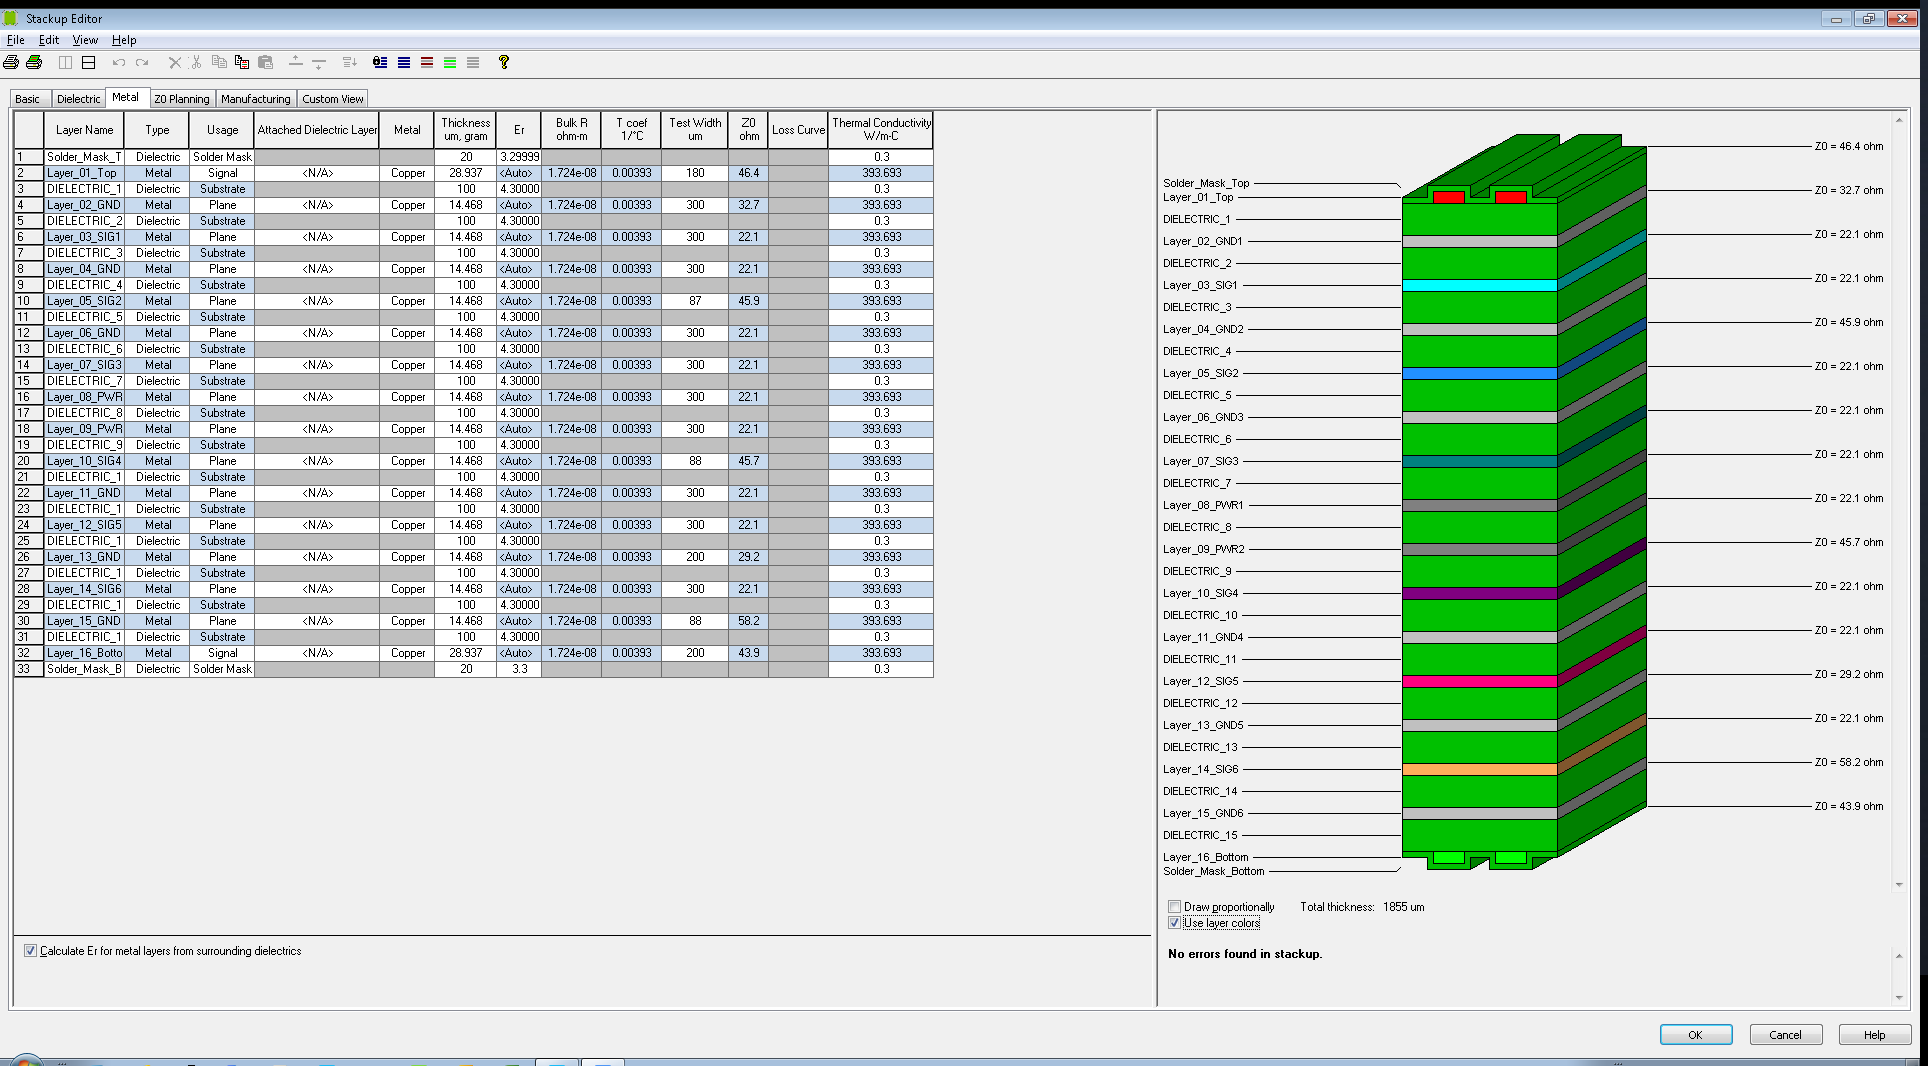
\includegraphics[width = \textwidth]{chap/04-work/img/stackup}
	\caption[Metal Layer Stackup]{Metal Layer stackup showing 16 layers.} 
	\label{fig:polaris}
\end{figure}

%https://industrial.panasonic.com/content/data/EM/PDF/ipcdatasheet\_R-5775.pdf
\subsection{Transmission lines}
%TODO
Transmission lines carry high-frequency signals, therefore the geometry of them is important, as this affects the impedance.
For single-ended the waveguide characteristic impedance should be \SI{50}{\ohm}, for differential signals \SI{100}{\ohm}.
For slow signals not that crucial, but for sensitive, high-speed signals, e.g. clock signals, proper calculation is very important to ensure signal integrity and reduce reflection and damping. 

For \glspl{pcb} usually coplanar waveguides are used for signal propagation.
The characteristic impedance depends from the dielectric, the trace width, separation between traces and separation between the signal traces and the ground planes/traces.
Formulas to calculate the characteristic impedance are quite lengthy and not easy to solve.
Therefore, tools exist to quickly calculate the geometric values needed for appropriate impedance.
For the design, the Si9000e \gls{pcb} field solver from \textit{Polar} (see \autoref{fig:polaris}) is used to calculate the necessary trace widths, separations, etc.

\begin{figure}[tbh]
	\centering
	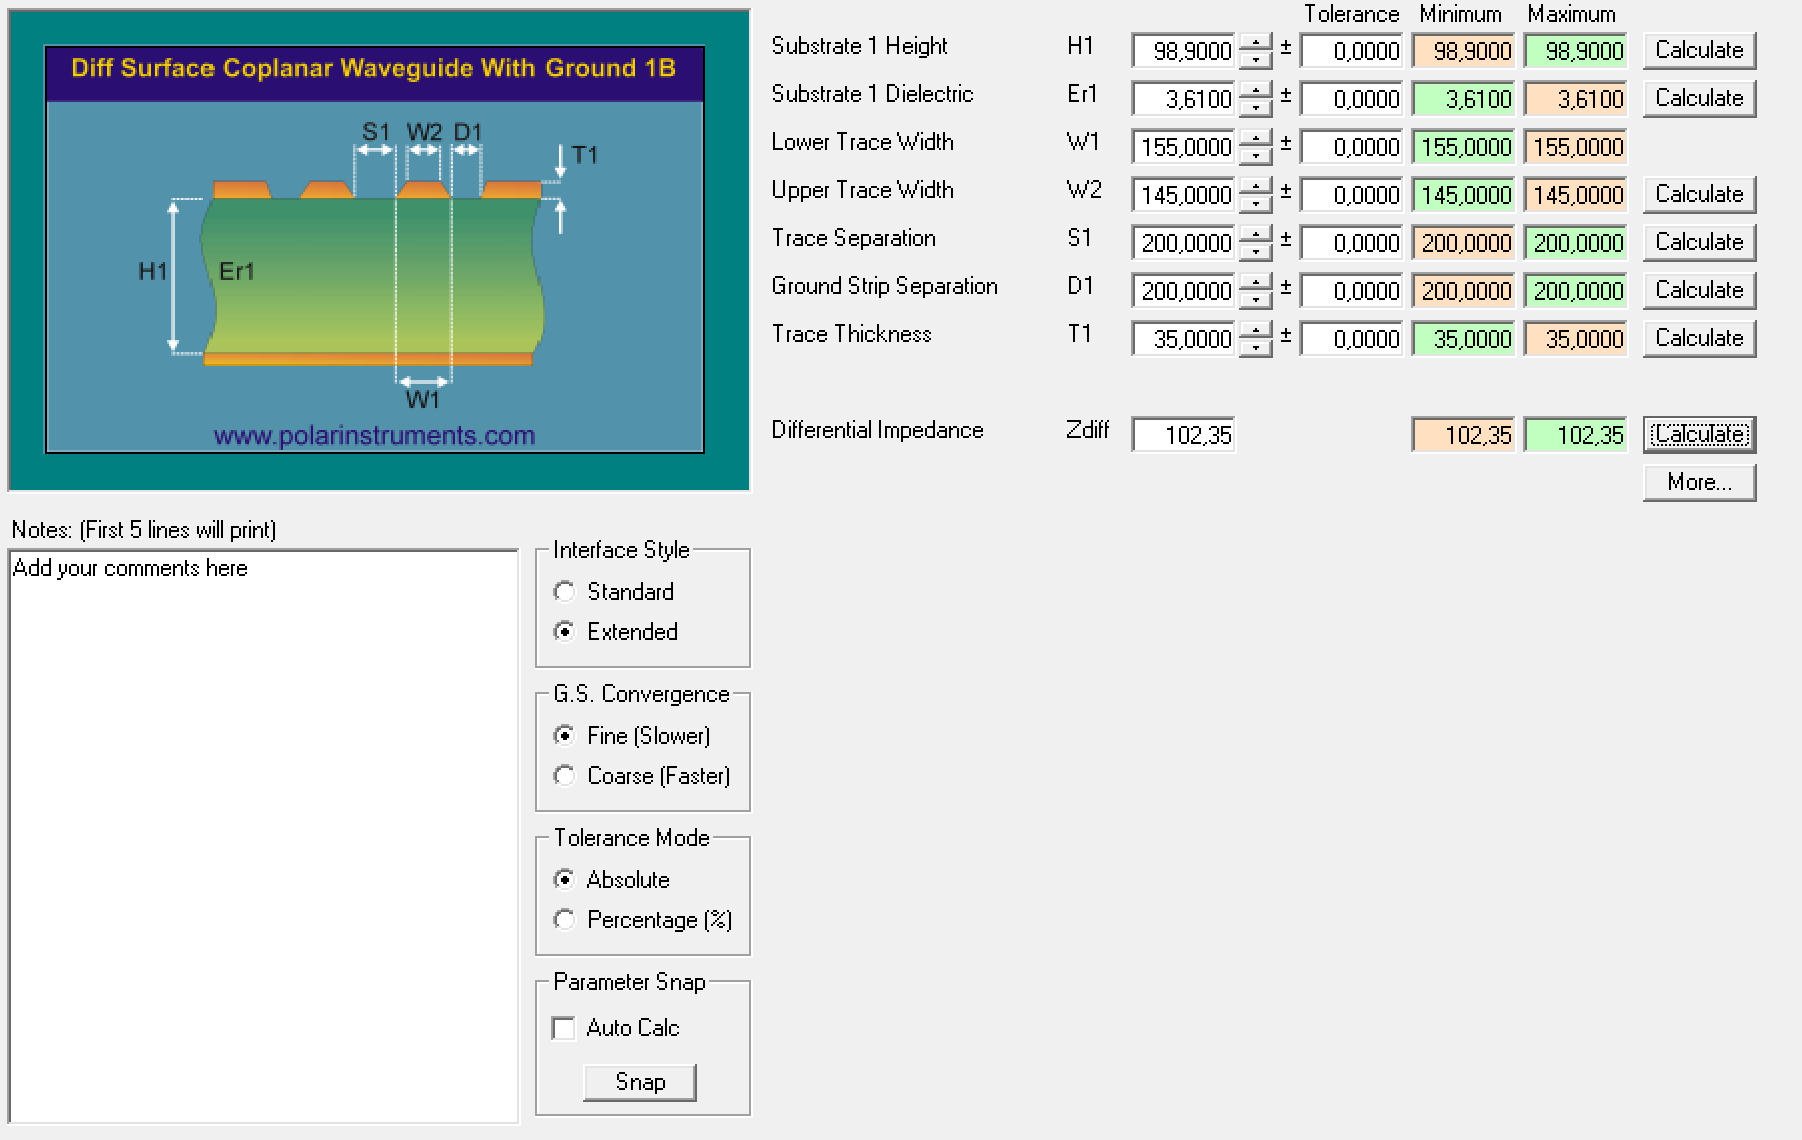
\includegraphics[width = \textwidth]{chap/04-work/img/polaris}
	\caption[Screenshot of the Polaris Si9000e]{Screenshot of the Polaris Si9000e, showing calculation of characteristic impedance} %todo screenshot, .. showing, ...
	\label{fig:polaris}
\end{figure}

Three geometries of waveguides are used in this design which are described in the following.
Furthermore, geometric dimensions calculated with the Si9000e tool are presented.

In principle, the geometries can be taken from the design of the sampling card of \gls{kapture} system, as these were specifically designed for 
As the dielectric constant of the substrate is slightly different (\gls{kapture}: 3.52, here: 3.61), the impedance has to be recalculated to check whether the characteristic value impedance still lies in the \SI{10}{\percent} tolerance.

\paragraph{Surface Coplanar Waveguide with Ground}
The surface coplanar waveguide has the geometry shown in \autoref{fig:microstrip_geometry}.
The single trace of thickness $t$ and width $a$ lies between two ground planes on a dielectric of thickness $h$ and the effective dielectric constant $\epsilon_r$.
Another ground plane is located at the bottom of the dielectric.
Separation between trace and ground plane is defined as $(b-a)/2 := d$. 

\begin{figure}[!htbp]
	\centering
	\includegraphics[width = \textwidth]{chap/04-work/img/cw}
	\caption{Coplanar Waveguide with Ground}
	\label{fig:microstrip_geometry}
\end{figure}

Trace width is assumed to be $a = \SI{180}{\micro\meter}$.
In the Si9000e tool, an upper and a lower trace width can be specified, therefore taking into account manufacturing processes.
As the exact upper trace width is not known, both are assumed to be \SI{180}{\micro\meter}.
Trace-To-Ground Separation, or "Ground Strip Separation", is defined by the manufacturing technology of the \gls{pcb} process: $d = \SI{250}{\micro\meter}$
With $h = \SI{98.9}{\micro \meter}$, $\epsilon_r = 3.61$ (at \SI{10}{\GHz}) this results in a characteristic impedance of \SI{52.90}{\ohm}. This lies well in the tolerance area. %todo of...

Over the frequency range, the value of the effective dielectric constant changes from 3.71 (at \SI{1}{\GHz}) to 3.61 (at \SI{10}{\GHz}).
As the tool provides the possibility to calculate the impedance versus a changing parameter, the influence of a changing dielectric was calculated. %todo which tool
As can be seen in \autoref{fig:surf_z0_vs_dk}, with higher effective dielectric constant, the characteristic impedance decreases (see \autoref{fig:surf_z0_vs_dk}).

\begin{figure}[tbh]
	\centering
	\includegraphics[width = \textwidth, height = 0.5\textwidth]{chap/04-work/img/TL/surf/surf_dk}
	\caption[Coplanar waveguide, $Z_o$ vs $\epsilon_r$]{Characteristic impedance $Z_o$ of a coplanar waveguide versus dielectric constant $\epsilon_r$}
	\label{fig:cwv_d1}
\end{figure}


The only parameters, which are not defined by the manufacturing process and therefore can be altered, are the ground strip separation $d$ and the trace width $a$.


\begin{figure}[tbh]
     \centering
     \begin{subfigure}[b]{\textwidth}
         \centering
         \includegraphics[width=\textwidth, height = 0.5\textwidth]{chap/04-work/img/TL/surf/surf_d1}
         \caption{$Z_o$ vs. ground strip separation $d$}
         \label{fig:surf_d1}
     \end{subfigure}
     
     \begin{subfigure}[b]{\textwidth}
         \centering
         \includegraphics[width=\textwidth, height = 0.5\textwidth]{chap/04-work/img/TL/surf/surf_w1}
         \caption{$Z_o$ vs. lower trace thickness}
         \label{fig:surf_w1}
     \end{subfigure}
     
     \begin{subfigure}[b]{\textwidth}
         \centering
         \includegraphics[width=\textwidth, height = 0.5\textwidth]{chap/04-work/img/TL/surf/surf_w2}
         \caption{$Z_o$ vs. upper trace width (assuming lower trace width $\SI{220}{\micro \meter}$) }
         \label{fig:surf_w2}
     \end{subfigure}
        \caption[Characteristic impedance of surface coplanar waveguide]{Characteristic impedance of surface coplanar waveguide versus different parameters}
        \label{fig:surf}
\end{figure}



\paragraph{Differential Pairs on Surface}
Some signals are propagated as differential pair traces on the \gls{pcb} surface.
Together with the surrounding ground plane and the ground plane on the layer below, these traces thus form the geometry of an edge-coupled coplanar waveguide (see \autoref{fig:eccw_geometry}). 
The formulas to calculate the characteristic impedance of this waveguide type is listed in \autoref{app:waveguides}.
\begin{figure}[tbh]
	\centering
	\includegraphics[width = \textwidth]{chap/04-work/img/eccw}
	\caption{Edge-Coupled Coplanar Waveguide}
	\label{fig:eccw_geometry}
\end{figure}

\begin{figure}[tbh]
	\centering
	\includegraphics[width = \textwidth, height = 0.5\textwidth]{chap/04-work/img/TL/surf_diff/surf_diff_dk}
	\caption]{$Z_o$ vs. dielectric constant $\epsilon_r$}
	\label{fig:cwv_d1}
\end{figure}


\begin{figure}[tbh]
     \centering
     \begin{subfigure}[b]{\textwidth}
         \centering
         \includegraphics[width=\textwidth, height = 0.5\textwidth]{chap/04-work/img/TL/surf_diff/surf_diff_w1}
         \caption{$Z_o$ vs. lower trace width}
         \label{fig:surf_d1}
     \end{subfigure}
     
     \begin{subfigure}[b]{\textwidth}
         \centering
         \includegraphics[width=\textwidth, height = 0.5\textwidth]{chap/04-work/img/TL/surf_diff/surf_diff_w2}
         \caption{$Z_o$ vs. upper trace thickness}
         \label{fig:surf_w1}
     \end{subfigure}
     
     \begin{subfigure}[b]{\textwidth}
         \centering
         \includegraphics[width=\textwidth, height = 0.5\textwidth]{chap/04-work/img/TL/surf_diff/surf_diff_s1}
         \caption{$Z_o$ vs. trace separation }
         \label{fig:surf_w2}
     \end{subfigure}
     \caption[Characteristic impedance of surface coplanar waveguide]{Characteristic impedance of surface coplanar waveguide versus different parameters}
        \label{fig:surf}
\end{figure}



\paragraph{Differential Pairs between Layers}
The analog signals from the \glspl{tha}, as well as the clock signals, are propagated through differential pair traces on the inner layers of the \gls{pcb}. 
This forms an offset coplanar waveguide as seen in \autoref{fig:docw_d1}.

\begin{figure}[tbh]
	\centering
	\includegraphics[width = \textwidth]{chap/04-work/img/docw.tikz}
	\caption{Offset Differential Coplanar waveguide}
	\label{fig:docw_d1}
\end{figure}


\subsection{Component Placement and Routing}

\paragraph{Component placement}
\begin{itemize}
\item connectors need to be placed exactly to match the connectors on the board. The connectors therefore define the geometry of the board in a large way.
\item Analog and digital part of the board are separated: topside is digital, bottomside is analog
\item For shielding purposes, layers are alternating: SIG-GND-SIG-GND-SIG-... This is important for differential pairs, as they should GND right below/above, because this serves as a return path (and as shielding from noise e.g. from digital signals)
\item Power planes are placed in such a way, that no or only few signal traces are routed above/below, as any switching signal may introduce noise on the power plane -> no stable voltage
\item decoupling capacitors are placed in such way, that big capacitor is connected to the power plane of the external ps/voltage regulator. The filtered power level is propagated to an innerlayer. The smaller bypass capacitor is connected to this layer by a via and to the power supply pin of the respective chip. The capacitor connects the component to the clean power plane and bypasses high frequency variations. The bypass capacitor is closed as close as possible to the power supply pin.
\item \glspl{tha} have been placed on the edge for better reaching
\item stitching vias are used to shield the sensitive \glspl{ic} as much as possible from EMI
\item delay chips have been arranged evenly so no further delay is introduced 
\item fanout buffer have been placed in the middle of two groups à 8 \glspl{tha} for even distribution of the signal
\item LMK04808B is placed right in the middle to evenly distribute clocking to the fanout buffers and the other to PLL.
\item LMX are placed close to the LMK and as close as possible to the corresponding LPAM connector.
\item Voltage regulators are placed symmetrically, this makes it easier to provide power planes in an efficient way.
\end{itemize}
